%!TEX root=../../main.tex
\begin{chapterpage}{Logistic Regression}
  \chaptertitle{Logistic Regression} \label{LogisticRegression}
  \chaptersection{chapterOverview}
  \chaptersection{introSimpleLogisticRegression}
  \chaptersection{inferenceSimpleLogisticRegression}
  \chaptersection{generalMultipleLogistic}
  \chaptersection{assessingModelFitMultipleLogisticRegression}
 \chaptersection{caseStudy}
  \chaptersection{notesLogisticRegression}
 \end{chapterpage}

\renewcommand{\chapterfolder}{ch_logistic_regression_oi_biostat}

\noindent%

%____________________

\noindent{\textit{NOTE: This supplement to the first edition is being released online as supplemental Chapter 9. Its pagination corresponds to the printed first edition text. This supplement includes a set of exercises and solutions to the odd-numbered exercises.}}

\chapterintro{Logistic regression is used to explore relationships between a response variable with two possible values (e.g., yes/no, success/failure, 0/1, etc.) and one or more predictor variables. The \term{logistic regression}  model estimates the odds of an outcome given a predictor, and the odds ratio (OR) associated with change in the value of a predictor; in certain cases, the model also estimates the probability of an outcome given a predictor.}   
%____________________

\setlength\parindent{20pt}

\section{Chapter overview}
\label{chapterOverview}

This chapter focuses on traditional methods of inference for logistic regression that are commonly used in epidemiology and public health, with emphases on both inference for model parameters and prediction.  The interpretation and use of logistic models for inference is contained in the three sections following this overview; these sections contain the core material used in many applications in medical research, epidemiology and public health.  

The last two sections describe methods for assessing the fit of a logistic model, both for inference and for prediction, and present an extended case study using logistic regression to modify and evaluate a triage system in hospital emergency departments.  The section on assessing fit is longer than most sections in the book, but the material is necessary for understanding the behavior of the  proposed triage system. Since model predictions are sometimes used as diagnostic tools, it is particularly important to understand the strengths and weaknesses of a model, as well as methods for estimating error rates.

Logistic regression relies heavily on software.  Even the simplest models cannot be fit by hand; direct formulas for parameter estimates and standard errors do not exist.  Consistent with earlier chapters, the treatment here emphasizes interpretation of both models and computer output for estimated models.  For students interested in working directly with data the chapter labs contain \textsf{R}-based exercises that illustrate how to fit and interpret models to data.

Logistic regression has also become an important tool in data exploration and detecting patterns in data and is now widely used in machine learning.  There is not space here to explore those ideas, but Chapter 9 of \textit{OpenIntro Statistics, 4th ed.} examines building a logistic regression explanatory model for possible bias in the review of resumes submitted for a listed job opening.  That material can serve as an introduction to data exploration with logistic regression.

\section{Introduction to simple logistic regression}
\label{introSimpleLogisticRegression}

\subsection{The model for simple logistic regression}

\index{data!hyperuricemia|(}

Hyperuricemia is the presence of abnormally high levels of uric acid in the blood, a  condition than can lead to kidney stones and gout; hyperuricemia may also be responsible for chronic kidney disease, cardiovascular disease, and other metabolic disorders. According to current criteria, men are diagnosed as having hyperuricemia if a uric acid measurement is at least as high as $416\mu\text{mol/L}$.  The cutoff for women is $360\mu\text{mol/L}$. Research suggests that risk of hyperuricemia is correlated with the consumption of red meat, seafood, and beans. Hyperuricemia is more common in high-income countries and economically developing countries with Western diets (characterized by high daily intake of saturated fats, animal protein, sodium, and refined sugars). The prevalence of hyperuricemia ranges between 15\% and 25\% in Asian countries. 

Hyperuricemia is present without symptoms approximately 30\% of the time, so it would be useful to identify clinical measurements indicative of hyperuricemia; i.e., measurements signaling that a patient should have their uric acid level tested.

Zeng, et al.\footfullcite{zeng2015association} report a cross-sectional study examining the association of hyperuricemia with dietary magnesium in 5,168 participants in China. The study measured several other possible predictors, including body mass index (BMI,measured in  $\text{kg/m}^2$.).  Some literature has suggested that BMI has a strong association with hyperuricemia in various populations. This section explores that relationship in a random sample of 500 participants from the Zeng study. The full dataset (\texttt{hyperuricemia}) and the random sample (\texttt{hyperuricemia.samp}) are in the data package \texttt{oibiostat}.

\begin{comment}

\begin{figure}[h!]
  \centering
  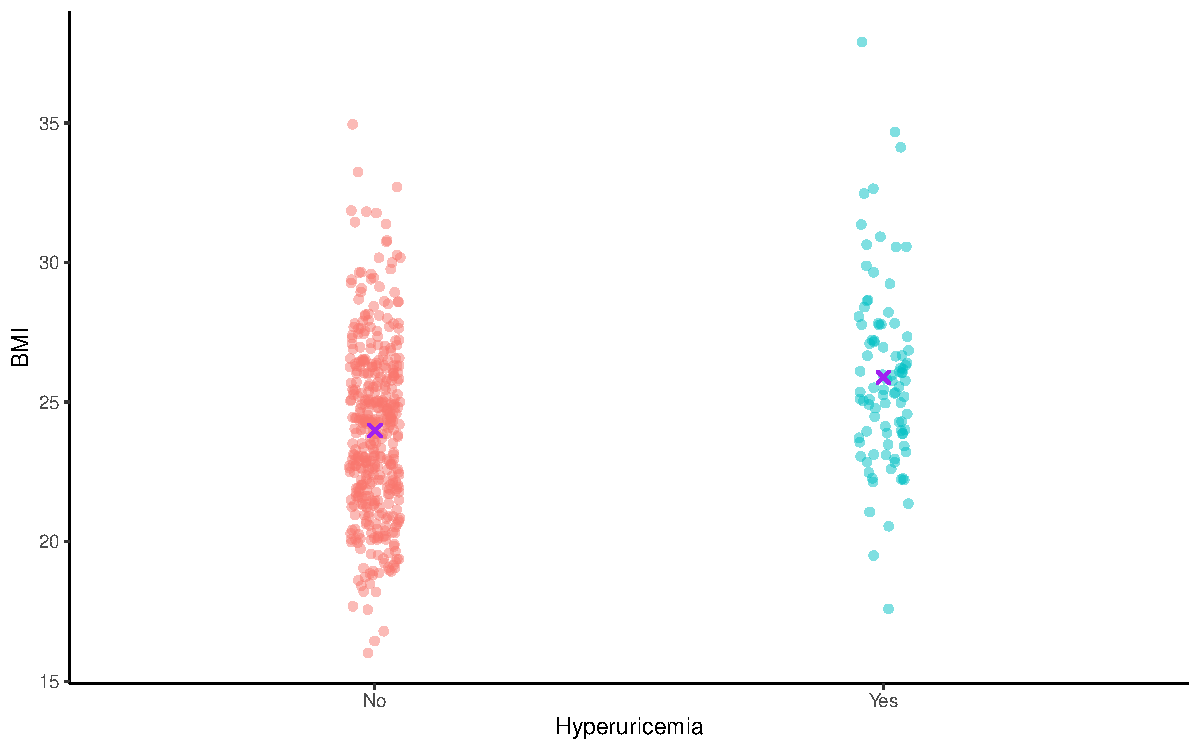
\includegraphics[width=0.80\textwidth]
  {ch_logistic_regression_oi_biostat/figures/bmiHuDotplot/bmiHuDotplot.pdf}
     \caption{Dot plots showing the distribution of BMI in participants without (labeled No) and with hyperuricemia (Yes).  The points have been jittered horizontally.}
     \label{figure:bmiHuDotplot}
 \end{figure}

The side by side dot plots in Figure~\ref{figure:bmiHuDotplot} show that in this study sample hyperuricemia tends to occur more often with larger values of BMI; the mean of BMI (marked by "x" in the plot) in the groups with and without hyperuricemia are, respectively, 25.9 and 24 $\text{kg/m}^2$. But the figure does not provide information about a relationship between individual values of BMI and the presence of hyperuricemia.  As with linear regression, it might is useful to explore that relationship in a scatterplot.

\end{comment}
 
Figure~\ref{figure:bmiHuProbSecondTileDataOnly} shows the presence  of hyperuricemia on the $y$-axis and BMI on the $x$-axis. The light blue dots represent $(x_i, y_i)$ pairs for each individual in the sample of 500, where $x_i$ is an individual's BMI and $y_i$ equals 0 (hyperuricemia absent) or 1 (hyperuricemia present). A small amount of random noise has been added to the $y$-values (referred to as "\term{jittering}") to make it easier to see where the points are most densely clustered.
        
     \begin{figure}[h!]
        \centering
        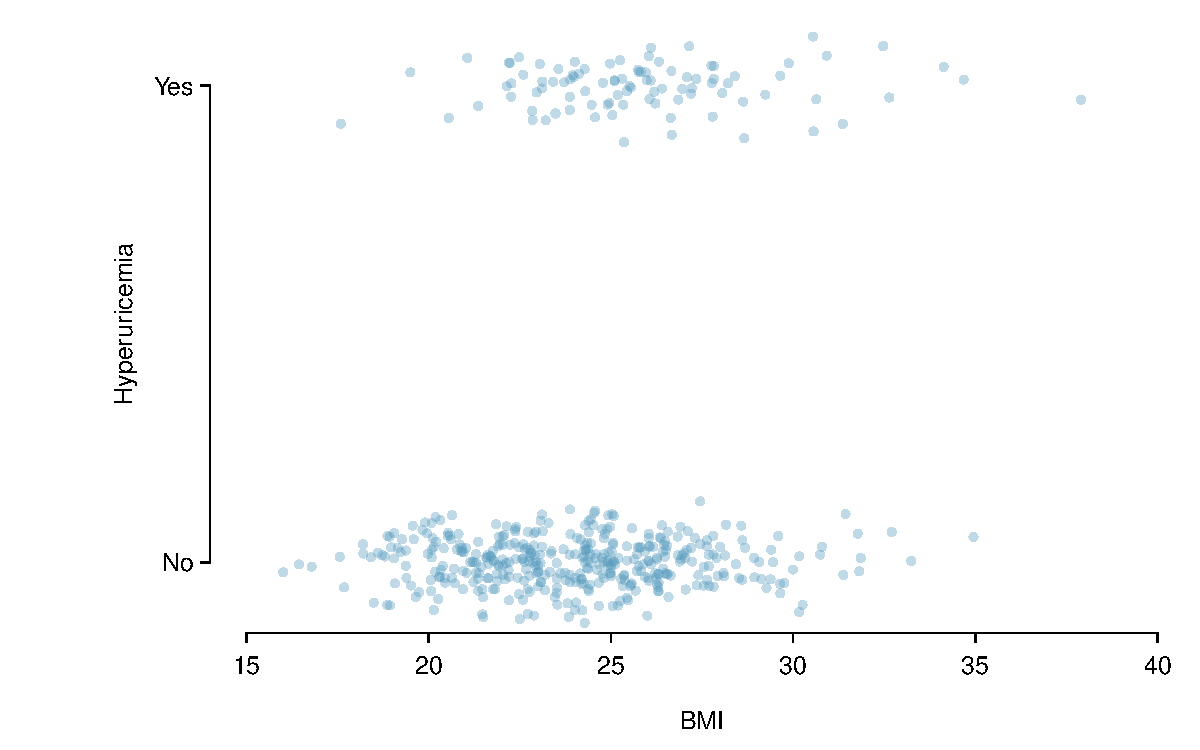
\includegraphics[width=0.80\textwidth]
        {ch_logistic_regression_oi_biostat/figures/bmiHuProbSecondTile/bmiHuProbSecondTileDataOnly.pdf}
         \caption{Presence of hyperuricemia versus BMI. For each case of $y_i = 1$ if hyperuricemia is present (labeled Yes on the vertical axis) and $y_i = 0$ if hyperuricemia is absent (labeled No). The $y$ values have been jittered. The mean BMI in each group is marked by an "x".}
         \label{figure:bmiHuProbSecondTileDataOnly}
     \end{figure}

The blue dots at $y = 0$ cluster between BMI values of about 17 to 30, while the dots at $y = 1$ are most concentrated around BMI 23 to 28, confirming that  hyperuricemia is associated with larger values of BMI. It still difficult, however, to see enough details to judge the strength of association from this plot. For example, while this plot clearly implies that an individual with BMI lower than 22 is unlikely to have hyperuricemia (since practically all points with BMI less than $22$ have $y = 0$), it is not clear how to judge the risk of hyperuricemia for individuals with moderate values of BMI, since points with BMI around $25$ exist at both $y = 0$ and $y = 1$.

Computing summary measures can provide further insight about the association between hyperuricemia and BMI.

\begin{examplewrap}
\begin{nexample}{The World Health Organization (WHO) labels $\text{BMI} \ge 30$ as obese and $25 \le \text{BMI} < 30$ as overweight or pre-obese\footnote{See Section~\ref{notesLogisticRegression} for a discussion on the use of these cut-points in Asian populations}. In the sample of 500 participants from the Zeng study, 204 individuals had $\text{BMI} \geq 25$. Of these individuals, 57 had hyperuricemia. Compute the probability and odds that a study participant with $\text{BMI} \ge 25$ has hyperuricemia.}\label{example:preobeseHyperurcemia}

    Among these 204 participants, if 57 had hyperuricemia then the estimated conditional probability of hyperuricemia in this group is $57/204 = 0.279$. Odds as a summary measure for binary data are discussed in Section~\ref{caseControlStudiesEstimates}. Briefly, the odds of an outcome is the ratio of the number of times an outcome occurs divided by the number of times it does not; thus, the odds of hyperuricemia in these 204 study participants equals $57/(204 - 57) = 0.388$.
\end{nexample}
\end{examplewrap}

In the sample of 500 individuals, 95 were hyperuricemic and 405 were not, so the estimated probability and odds of hyperuricemia based on the sample of 500 are $95/500 = 0.190$ and $95/405 = 0.235$, respectively.  An individual drawn at random from the entire study sample has a lower probability of being hyperuricemic than an individual drawn at random from the participants with  $\text{BMI} \geq 25$: probability 0.235 versus 0.279. Thus, these data suggest an association between BMI and hyperuricemia; specifically, that larger BMI is associated with increased risk of hyperuricemia. This is consistent with the trend visible in Figure~\ref{figure:bmiHuProbSecondTileDataOnly}.

Figure~\ref{figure:huBMIQuintiles} shows the prevalence of hyperuricemia by quintile of BMI.  Quintiles divide the study sample into five groups of equal size, so each row of the table has 100 observations. With increasing BMI quintile, the estimated probability and odds of hyperuricemia increase. In the lowest quintile, in which average BMI is 20.08, the probability of hyperuricemia is $0.05$ and the odds of hyperuricemia are $0.053$. In the highest quintile, in which average BMI is 28.92, the probability and odds of hyperuricemia are larger: $0.32$ and $0.471$, respectively.

Probabilities and odds are not identical but they provide similar information. Odds and probabilities increase or decrease together, and one can be calculated from the other.  If $p$ is the probability of an event, $p/(1 - p)$ are the odds.  Algebra can be used to show that $p = \textrm{odds} / (1 + \textrm{odds})$.

% latex table generated in R 4.0.2 by xtable 1.8-4 package
% Tue Sep 29 12:37:16 2020
% column names and legend have been edited directly
%\begin{table}[ht]
\begin{figure}[ht]
\centering
\begin{tabular}{cc|cc|cc}
  \hline
  \textbf{BMI Quintile} & \textbf{Mean BMI} & \textbf{HU Absent} & \textbf{HU Present} & \textbf{Est. Probability} & \textbf{Est. Odds} \\
  \hline
  1 & 20.08 & 95 & 5 & 0.05 & 0.053 \\
  2 & 22.55 & 85 & 15 & 0.15 & 0.176 \\
  3 & 24.32 & 82 & 18 & 0.18 & 0.220 \\
  4 & 25.84 & 75 & 25 & 0.25 & 0.333\\
  5 & 28.92 & 68 & 32 & 0.32 & 0.471\\
   \hline
\end{tabular}
\caption{Hyperuricemia (HU) by quintiles of BMI. Each row provides information within a specific BMI quintile: average BMI, number of individuals with and without hyperuricemia, and the estimated probability and estimated odds of hyperuricemia.}
\label{figure:huBMIQuintiles}
%\end{table}
\end{figure}


\begin{exercisewrap}
\begin{nexercise}
  Using the algebraic relationship between probability and odds, show that if the probability of hyperuricemia is $0.05$, the odds of hyperuricemia are $0.053$. Additionally, show that if the odds of hyperuricemia are $0.471$ then the probability equals $0.32$.\footnotemark{}
\end{nexercise}
\end{exercisewrap}
\footnotetext{If $p = 0.05$, compute the odds as $p/(1-p) = 0.05/(1 - 0.05) = 0.053$. If the odds are $0.471$, compute the probability as $\text{odds}/(1 + \text{odds}) = 0.471/(1 + 0.471) = 0.32$. }

Dividing the study sample into smaller groups and computing summary measures will provide more detail about how risk of hyperuricemia varies with individual BMI values. The dark blue circles in Figure~\ref{figure:bmiHuProbSecondTile} represent information obtained from grouping individuals into $2^{nd}$-percentiles, just as Figure~\ref{figure:huBMIQuintiles} groups individuals by every $20^{th}$ percentile; i.e., the 500 cases have been split into 50 groups of 10 cases per group. Each dark blue circle has $x$-value equal to the mean BMI within the group and $y$-value equal to the proportion of individuals with hyperuricemia within the group. The dark blue circles more clearly demonstrate that larger BMI tends to be associated with increased estimated probability of hyperuricemia than the light blue circles representing the observed data.

\begin{figure}[h!]
	\centering
	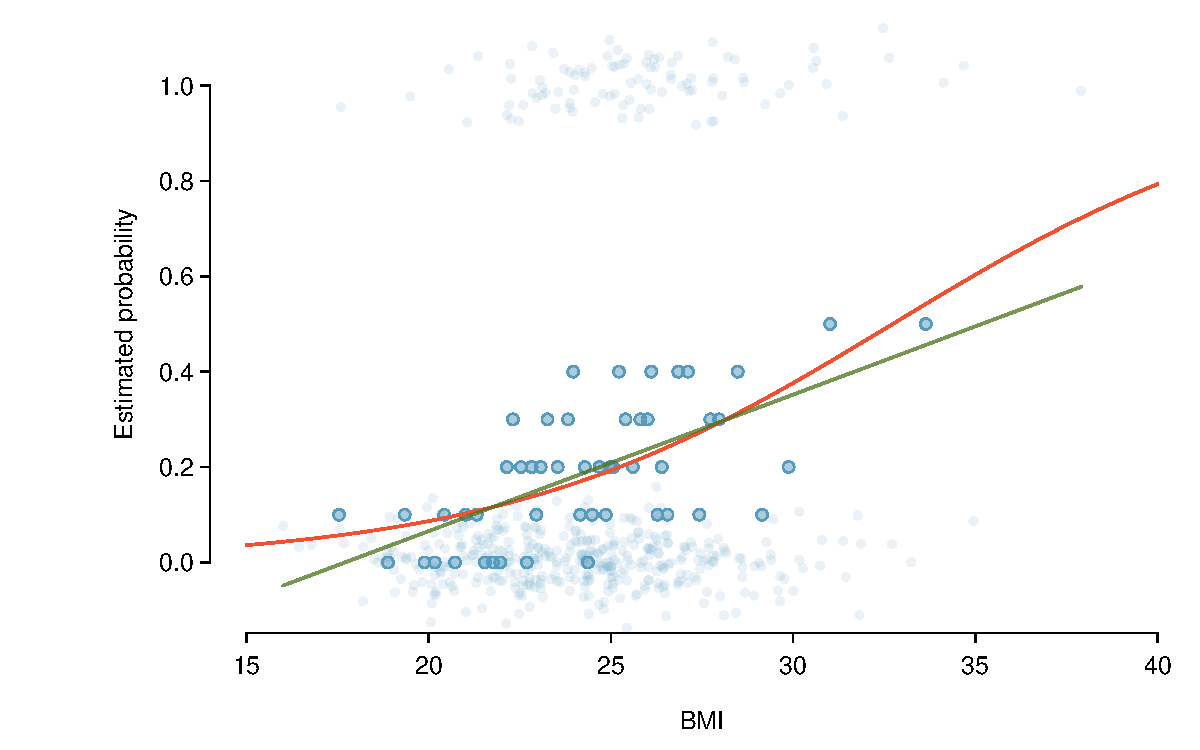
\includegraphics[width=0.80\textwidth]
	{ch_logistic_regression_oi_biostat/figures/bmiHuProbSecondTile/bmiHuProbSecondTile.pdf}
    \caption{Estimated probability of hyperuricemia versus BMI. The small light blue dots show observed $(x_i, y_i)$ pairs. Each large blue dot represents the proportion of individuals with hyperuricemia in each $2^{nd}$-percentile; i.e., each group when the sample is divided into 50 groups based on BMI. The green line is the least squares model for hyperuricemia versus BMI. The red curve is a logistic model for hyperuricemia versus BMI.}
    \label{figure:bmiHuProbSecondTile}
\end{figure}

The green line in Figure~\ref{figure:bmiHuProbSecondTile} is the least squares line for a model predicting hyperuricemia from BMI. Since the mean of a binary variable taking on values 0 and 1 equals the estimated probability of the variable taking on the value 1 (i.e., the proportion of times that $y = 1$), the linear model estimates the probability of hyperuricemia at each value of BMI. While the line mostly fits the data reasonably well, it shows a lack of fit at the smallest BMI values where it predicts probabilities less than 0. 

The least squares line in Figure~\ref{figure:bmiHuProbSecondTile} is based on the model
\begin{align*}
  E(Y_i) &= P(Y_i = 1) \\
         &= \beta_0 + \beta_1 (\text{bmi}),
\end{align*}
where $Y_i$ has value 1 when hyperuricemia is present and 0 otherwise.  The green line drops below 0 for the smaller values of BMI because the linear model does not restrict predicted values to lie between 0 and 1.  The red curve, which shows a model-based estimate of the probability of hyperuricemia using logistic regression, is a better fit to the data across the range of BMI values. 

\begin{comment}
\begin{exercisewrap}
\begin{nexercise}
  Compute the odds and log odds for the probabilities $0.01, 0.10, 0.50, 0.95$ and $0.99$.\footnotemark{}
\end{nexercise}
\end{exercisewrap}
\footnotetext{For a probability $p$, use the formula $\text{odds} = p/(1-p)$. For probability $0.01$ the odds and log odds are respectively, $0.010$ and $-4.595$. For $0.10$, the odds and log odds are $0.111$ and $-2.197$.  For $0.50$, the odds and log odds are $1$ and $0$.  For $0.95$, the odds and log odds are $19$ and $2.944$.  For $0.99$, the odds and log odds are $99$ and $4.595$.}

\end{comment}

Suppose $E$ is an event, $x$ is a predictor, and $p_{E}(x)$ is the conditional probability of $E$ given $x$. The odds of $E$ given $x$ are $p_{E}(x)/(1 - p_{E}(x))$\index{odds}. The simple logistic regression model\index{simple logistic regression} for the odds of $E$ given $x$ is a linear model on the log(odds) scale. Just as in least squares linear regression, the right-hand side of the model is a linear combination of parameters (the intercept and slope) and $x$: 
\begin{align}
   \log\left(\frac{p_{\text{E}}(x)}
  {1 - p_\text{E}(x)}\right) &= \beta_0 + \beta_1 x,
  \label{eqn:logOddsLogisticRegression}
\end{align}
or, equivalently,
\begin{align}
 \log(\text{odds}_\text{E}(x)) &= \beta_0 + \beta_1 x.
   \label{eqn:logOddsLogisticRegressionEquiv}
\end{align}

Exponentiating both sides of Equation~\ref{eqn:logOddsLogisticRegressionEquiv} yields
\begin{align}
  \text{odds}_\text{E}(x)) &= \exp(\beta_0 + \beta_1 x) \notag \\
  &= \exp(\beta_0) \exp(\beta_1 x).
    \label{eqn:oddsLogisticRegression}
\end{align}

If $Y$ is a binary variable with value 1 when $E$ occurs and 0 otherwise,
Equation~\ref{eqn:oddsLogisticRegression} is a model for the odds that $Y = 1$, given $x$.

Probabilities can be estimated using the relationship \index{simple logistic regression!estimating probabilities}

\begin{align}
  p_{E}(x) &= \frac{\text{odds}_{E}(x)}{1 + \text{odds}_{E}(x)} \notag \\
        &= \frac{\exp(\beta_0 + \beta_1 x)}
        {1 + \exp(\beta_0 + \beta_1 x)}.
        \label{eqn:probLogisticRegression}
 \end{align}

Software used to estimate logistic regression usually provides estimates for log(odds) in the form of Equation~\ref{eqn:logOddsLogisticRegression}, and the conversion to odds or probabilities is done with either a separate step in the program or by hand.

\begin{exercisewrap}
  \begin{nexercise}\label{guidedPracticeSimpleModel} \index{!hyperuricemia}
Suppose the logistic regression model for an event $E$ is given by
\begin{align*}
\log(\text{odds}_\text{E}(x)) &= \beta_0 + \beta_1 x \\
             &= 0.5 - 0.75x.
\end{align*}
Calculate the odds and probability of $E$ when $x = 1.0$.
\footnotemark{}
\end{nexercise}
\end{exercisewrap}
\footnotetext{The log(odds) are $0.5 - 0.75(1) = -0.25$, so the odds and probability are, respectively, $\exp(-0.25) = 0.779$ and $0.779/(1 + 0.779) = 0.438$.}

Computer algorithms that estimate the parameters in logistic regression use the method of \term{maximum likelihood}\index{maximum likelihood}.  Since a logistic regression model can be converted to a model for the probability of an event $E$ given set of predictors, these probabilities can be used to write an algebraic expression for the probability of a set of observed responses given the predictors (details shown in more advanced courses).  This expression is called the likelihood of the data; the method of maximum likelihood selects estimates for $\beta_0$ and $\beta_1$ that make the likelihood as large as possible.

The estimated logistic regression model shown in the red curve in Figure~\ref{figure:bmiHuProbSecondTile} is explored in Section~\ref{section:analyzingHyperuricemia}.

The log in Equation~\ref{eqn:logOddsLogisticRegression} is $\log_e$, the natural logarithm function.  Since the natural log is used often in statistics, the subscript $e$ is usually omitted. The transformation $\log(\frac{p}{1-p})$ has its own name, the \term{logit function}.\footnote{Specifically, $\text{logit}(p) = \log(\frac{p}{1-p})$.}

\newpage
\subsection{Interpreting model parameters}
\index{simple logistic regression!model parameters}

Figure~\ref{figure:probVsPredictor} shows the relationship between probability and the value of a predictor $x$ for four different models of the form specified by Equation~\ref{eqn:probLogisticRegression}. The model coefficients ($\beta_0, \beta_1$) are (-3.0, 0.6) for the solid line, (-3.0, 0.8) for the dashed line, (3.0, -0.6) for the dotted line, and (-0.4, 0.0) for the horizontal line.

The model parameter $\beta_1$ determines the relationship between predicted probabilities and values of the predictor $x$. The solid and dashed lines show a positive association; when $\beta_1 > 0$, probabilities increase with increasing values of the predictor $x$. Since odds and probabilities increase together, positive values of $\beta_1$ indicate that the odds of an event increase with increasing values of $x$. A larger positive value for $\beta_1$ indicates of a stronger positive association. The dashed line, which has a larger $\beta_1$ than the solid line, shows a steeper incline in the center of the graph. Probabilities change more rapidly with changing values of $x$. The dotted line shows a negative association; when $\beta_1 < 0$, probabilities and odds decrease with increasing values of $x$. Probability starts out near 1 when $x$ is small, then decreases to near 0 once $x$ increases to 10. The horizontal line with $\beta_1 = 0$ shows no association between the event and values of x.

% figure placement is a problem.  LaTeX is forcing it below the subsection break so I inserted a page break at the beginning of the subsection.  It could just as well go at the end of the subsection after the figure.

\begin{figure}[!htb]
	\centering
	\includegraphics[width=0.70\textwidth]
	{ch_logistic_regression_oi_biostat/figures/probVsPredictor/probVsPredictor.pdf}
    \caption{Probability versus a predictor $x$ for four models of the form specified by Equation~\ref{eqn:probLogisticRegression}. The model coefficients ($\beta_0, \beta_1$) are (-3.0, 0.6) for the solid line, (-3.0, 0.8) for the dashed line, (3.0, -0.6) for the dotted line, and (-0.4, 0.0) for the horizontal line.}
    \label{figure:probVsPredictor}
\end{figure}


\subsection{Hyperuricemia and BMI}
\label{section:analyzingHyperuricemia}

If $E$ is hyperuricemia and $x = \text{bmi}$, the logistic regression model for the association between hyperuricemia and BMI is
\begin{align*}
  \log\left[\frac{p(E|\text{bmi})}{1-p(E|\text{bmi})}\right] &=  \beta_0 + \beta_1 (\text{bmi}),
\end{align*}
or, equivalently,
\begin{align}
  \log(\text{odds}_\text{E}(\text{bmi})) &=  \beta_0 + \beta_1 (\text{bmi}).
   \label{eqn:hyperuricemiaBmiLogit}
\end{align}

Figure~\ref{figure:bmiHyperuricemiaLogRegCoeff} shows the result of using \textsf{R} to estimate the coefficients in Equation~\ref{eqn:hyperuricemiaBmiLogit}.  The `Intercept' is the estimate $b_0$  of $\beta_0$ and the term labeled `bmi' is the estimate $b_1$ of $\beta_1$.

\begin{figure}[ht]
\centering
\begin{tabular}{rrr}
  \hline
 & Intercept & bmi  \\
  \hline
 & -6.054 & 0.185  \\
   \hline
\end{tabular}
\caption{Estimated logistic regression coefficients for the association of hyperuricemia with BMI.}
\label{figure:bmiHyperuricemiaLogRegCoeff}
\end{figure}

Expressed algebraically, the estimated model is
\begin{align}
  \log(\widehat{\text{odds}}_\text{E}(\text{bmi})) &= -6.054 + 0.185 (\text{bmi}).
  \label{eqn:bmiHyperuricemiaModel}
\end{align}

The red curve in Figure~\ref{figure:bmiHuProbSecondTile} is drawn using this estimated model after log(odds) were converted to probabilities, just as in Guided Practice~\ref{guidedPracticeSimpleModel}. For example, a member of the study population with BMI 30.0 has an estimated log(odds) of hyperuricemia of $-6.054 + (0.185)(30) = -0.504$. To compute the odds, exponentiate the estimated log odds: $\exp(\log(\widehat{\text{odds}})) = \exp(-0.504) = 0.604$. Then, convert from odds to probability: the predicted probability of hyperuricemia for an individual with BMI 30.0 is $0.604/(1 + 0.604) = 0.377$. If these data represent a random sample from a large population, about 38\% of individuals with $\text{BMI} = 30$ are predicted to have hyperuricemia.

Just as with $2 \times 2$ tables, probabilities can be estimated with logistic regression in either cross-sectional studies or studies with exposure based sampling; the hyperuricemia study was a cross-sectional study, so probabilities can be estimated using the estimated model. This issue is discussed in detail for $2 \times 2$ tables in Section~\ref{designVsAnalysisBinaryData} in the web supplement and is part of the assumptions for logistic regression listed in Section~\ref{inferenceSimpleLogisticRegression}.

The coefficient $0.185$ has an interpretation similar to a slope in linear regression: every one unit change in BMI is associated with an additive increase of $0.185$ in the log odds of hyperuricemia.

\begin{examplewrap}
\begin{nexample}{Suppose two members of the study population have BMI values $30.0$ and $33.2$. What is the estimated relative odds for hyperuricemia (i.e., the odds ratio), comparing the individual with BMI = 33.2 to the one with BMI = 30.0?}\label{example:ORHyperuricemia33v30}
When BMI = 33.2, the estimated log odds of hyperuricemia are
\begin{align*}
  \log[\widehat{\text{odds}}_E(\text{bmi} = 33.2)] = -6.054 + (0.185)(33.2) = 0.088,
\end{align*}
and the estimated odds of hyperuricemia are $\exp(0.088) = 1.092$. The estimated odds of hyperuricemia for an individual with BMI $30.0$ are $0.604$ (calculated earlier).

The estimated OR comparing these two individuals is $1.092/0.604 = 1.808$.  The odds of hyperuricemia are estimated to be 1.8 times as large for an individual with BMI~33.2 versus an individual with BMI~30.0.  This model is consistent with the data in Figure~\ref{figure:huBMIQuintiles} and suggests there is indeed a strong association between BMI and the odds of hyperuricemia, as others have found.  The tools of inference discussed in Section~\ref{inferenceSimpleLogisticRegression} will show that this association is stronger than would be expected by chance alone under the assumption the null hypothesis of no association is true.
  \end{nexample}
\end{examplewrap}

\index{odds ratio}


Odds ratios can be calculated directly from the coefficients in the model. Since the model for logistic regression is
\begin{align*}
  \log(\text{odds}(x)) = \beta_0 + \beta_1 x,
\end{align*}
the difference in log odds for two values $x_1$ and $x_2$ is
\begin{align*}
  \log[\text{odds}(x_2)] - \log[\text{odds}(x_1)] &= \beta_1(x_2 - x_1).
\end{align*}
The relationship
\begin{align*}
  \log(b) - \log(a) = \log(b/a)
\end{align*}
implies that
\begin{align*}
  \log\left[\frac{\text{odds}(x_2)}{\text{odds}(x_1)}\right] = \beta_1(x_2 - x_1)
\end{align*}
and
\begin{align}
  \frac{\text{odds}(x_2)}{\text{odds}(x_1)} = \exp[\beta_1(x_2 - x_1)].
  \label{eqn:oddsRatioLogisticRegression}
\end{align}

Suppose two members of a population have BMI values given by $x_1=\text{bmi1}$ and $x_2 = \text{bmi2}$. The estimated odds ratio comparing these two individuals is
\begin{align*}
  \widehat{\text{OR}} &= \text{odds(bmi1)/odds(bmi2)} \\
  &= \exp[0.185(\text{bmi2} - \text{bmi1})].
\end{align*}

If two values of BMI differ by 1, the odds ratio (OR) will be $e^{0.185} = 1.20$. For every one unit increase in \texttt{bmi}, the odds changes by a factor of $1.20$. When calculating a change in odds using the model coefficients, the intercept plays no role, just as in similar calculations in linear regression.  More generally, in the model in Equation~\ref{eqn:logOddsLogisticRegression}, $\beta_1$ and $\exp(\beta_1)$ are, respectively, the difference in log(odds) and the OR between two cases when $x$ changes by 1 unit.

\begin{exercisewrap}
\begin{nexercise}
  Suppose two members of the study population have a BMI of 26 and 28, respectively.  Calculate the odds of hyperuricemia for each of them using
model~\ref{eqn:bmiHyperuricemiaModel}.  Calculate the relative odds (i.e., odds ratio) for an individual with BMI 28 compared to BMI 26.
\footnotemark{}
\end{nexercise}
\end{exercisewrap}
\footnotetext{The odds of hyperuricemia for the two individuals are $\exp[-6.054 + (0.185)(26)] = 0.288$ and $\exp[-6.054 + (0.185)(28)] = 0.417$. The relative odds are $0.417/0.288 = 1.45$.}

\begin{exercisewrap}
  \begin{nexercise}
    Calculate the relative odds of hyperuricemia for the two individuals with BMI 26 and 28 by using the coefficients in the logistic regression model directly, i.e., without calculating the individual odds.
    \footnotemark{}
  \end{nexercise}
\end{exercisewrap}
\footnotetext{Using the model coefficient, the relative odds is $\exp[(2)(0.185)] = 1.45$.}

The model can also be used to estimate prevalence ratios as discussed in Section~\ref{introAndTerminologyForRisk}.

\begin{examplewrap}
  \begin{nexample}{What is the estimated prevalence (i.e.\ probability) of hyperuricemia for two individuals with BMI $30.0$ and $33.2$? What is the estimated prevalence ratio for hyperuricemia, comparing the individual with BMI = $33.2$ to the one with BMI = $30.0$?}\label{example:RRHyperuricemia33v30}
    As mentioned earlier, the hyperuricemia data were collected in a cross-sectional study, so probabilities can be estimated (estimated probabilities were used to construct the red curve in Figure~\ref{figure:bmiHuProbSecondTile}).

    For these two individuals, the estimated probabilities of hyperuricemia are
\begin{align*}
  \hat{p}_E(33.2) &=\frac{1.092}{1 + 1.092} \\
            &= 0.522
\end{align*}
and
\begin{align*}
  \hat{p}_E(30.0) &=\frac{0.604}{1 + 0.604} \\
            &= 0.377.
\end{align*}
The prevalence ratio, comparing the participant with BMI = $33.2$ to the one with BMI = $30.0$ is $0.522/0.377 = 1.38$; the prevalence of hyperuricemia for individual with BMI = $33.2$ is estimated to be almost $1.4$ times ($40\%$ larger) that of the individual with the lower BMI.  Using the language of 
Section~\ref{inferenceBinaryData}, the relative risk of hyperuricemia for an individual with a BMI of $33.2$ vs $30.0$ is approximately $1.4$.
  \end{nexample}
\end{examplewrap}

\subsection{Checking model fit, hyperuricemia and BMI}
\label{assessingFitHyperuricemiaBMI}

This section describes a graphical method for checking the fit of a logistic model with a single continuous predictor, such as BMI. Methods for checking fit that use the inferential properties of logistic regression are discussed in Section~\ref{assessingModelFitMultipleLogisticRegression}.

Figure~\ref{figure:probVsObsHuBMI} shows values of the outcome variable $Y = 0$ (no hyperuricemia) or $Y = 1$ (hyperuricemia) plotted against model predicted probabilities. It is the analogue of plotting observed versus predicted values in linear regression, but because all the observed values are clustered at 0 or 1, it is less useful as a diagnostic than in linear regression.  As noted earlier, close inspection of the plot indicates that larger predicted probabilities tend to have a increased frequency of $Y = 1$, but the trend is subtle.

\begin{figure}[!tbh]
  \centering
  \includegraphics[width=0.70\textwidth]
  {ch_logistic_regression_oi_biostat/figures/probVsObsHuBMI/probVsObshuBMI.pdf}
    \caption{Predicted probabilities versus observed values of hyperuricemia. }
    \label{figure:probVsObsHuBMI}
\end{figure}

Grouping observations reduces the variability in a plot and can sometimes be helpful in checking a model. Figure~\ref{figure:predVsObsHuBMI} shows the same plot as in Figure 9.6, but with the addition of summary statistics computed within 10 equally sized buckets of size 50.  Each group is formed based on the predicted probability of hyperuricemia. For instance, the left-most point represents the group consisting of the 50 cases with the smallest predicted probabilities of hyperuricemia based on the model, which range between 0.043 to 0.091. Within this group, 2 individuals (a proportion of $2/50 = 0.04$) were hyperuricemic and the average predicted probability was $0.076$, so the point is at $(0.076, 0.040)$.  The vertical lines show $95\%$ confidence intervals for each estimated proportion.  If the logistic regression is a good fit, the estimated proportions and average predicted probabilities should be similar in each decile; the dashed line $y = x$ shows the extent to which the observed proportions and predicted probabilities agree.  Since all of  the confidence intervals touch the dashed line, the model seems to fit reasonably well.

With larger datasets, it is possible to obtain a clearer picture of the fit by increasing the number of buckets and/or the number of observations in each bucket. 

\begin{figure}[!tbh]
  \centering
  \includegraphics[width=0.70\textwidth]
  {ch_logistic_regression_oi_biostat/figures/predVsObsHuBMI/predVsObsHuBMI.pdf}
    \caption{Predicted probabilities versus observed proportions, with data grouped according into 10 equal sized buckets of predicted probabilities. The light blue dots at  $y = 0$ and $y = 1$ denote observed values of hyperuricemia (0 = "No", 1 = "Yes") plotted against predicted probabilities.}
    \label{figure:predVsObsHuBMI}
\end{figure}

Figure~\ref{figure:predVsObsHuBMI} is a type of \term{calibration plot} \index{calibration plot} discussed in more detail in Section~\ref{assessingModelFitMultipleLogisticRegression}.


\index{data!hyperuricemia|)}
%____________________


\section{Inference for simple logistic regression} \label{inferenceSimpleLogisticRegression}

How strong is the evidence for the association between BMI and hyperuricemia?

All models estimated from data have inherent uncertainty in the estimated parameters.  The standard errors of estimated parameters are a reminder to pay attention to the margin of error of statistical estimates.  Just as in linear regression, standard errors are used to calculate test statistics and confidence intervals.

Confidence intervals and tests for parameters in simple logistic regression will be valid if the assumptions behind the model are met, at least approximately.

\index{simple logistic regression!model assumptions}

\begin{onebox}{Assumptions for simple logistic regression} \label{box:logisticRegressionConditions}
  Let $E$ be an event and $Y$ a binary response variable that is 1 if $E$ has occurred and 0 if not. Let $X$ be a predictor thought to be related to the occurrence of $E$. A sample of observations $(x_1, y_1), (x_2, y_2)\ldots(x_n, y_n)$ can be used to estimate the log(odds) of the occurrence of $E$ (equivalently that $Y = 1$)  given $X = x$ using model~\ref{eqn:logOddsLogisticRegression} under the following conditions:

  \begin{enumerate}
      \item The logistic transformation is thought to be a reasonable model for the dependence of conditional probability or odds for the response variable given the predictor.
      \item The observations are independent pairs, i.e., no single pair depends on any of the others.
      \item If the sample was drawn using exposure-based or cross-sectional sampling, the conditional odds and probability of $E$ given $x$ can be estimated using relationships~\ref{eqn:oddsLogisticRegression} and ~\ref{eqn:probLogisticRegression}.  These estimates can be used to estimate odds and prevalence ratios.
      \item If the data are from a case-control study (i.e., outcome-based sampling) in which the sampling did not depend on exposure, conditional odds can be estimated but conditional probabilities cannot. Odds ratios can be estimated from the model, but prevalence ratios cannot.
  \end{enumerate}
\end{onebox}

Assumption 1 is more difficult to check than the usual linearity assumption in linear regression, but for continuous predictors such as BMI, scatterplots such as Figure~\ref{figure:bmiHuProbSecondTile} or Figure~\ref{figure:probVsObsHuBMI} can be helpful. Other diagnostic plots can be found in more advanced texts. For binary predictors, the model is generally reasonable.

Assumptions 2 - 4 depend on the study design. Assumption 2 is the standard assumption of independent observations.  Assumptions 3 and 4 are analogous to the connection between study design and parameters that can be estimated in an analysis of $2 \times 2$ tables, where the usual calculation of risk ratio leads to a biased estimate in case-control studies.  The formula for transforming an odds to a probability in a logistic model can be calculated but leads to incorrect estimates of probabilities.  Section~\ref{designVsAnalysisBinaryData} contains a discussion of this issue in $2 \times 2$ tables.

In the logistic model given by Equation~\ref{eqn:logOddsLogisticRegression}, a test of the null hypothesis $\beta_1 = 0$ is a test of no association between the predictor $x$ and the odds or the probability of $E$; i.e., a test of the null hypothesis that $x$ provides no information for predicting $E$.

As with all statistical models, tests and intervals are based on the sampling distributions of estimated parameters.

\index{sampling distribution!simple logistic regression coefficient}

\begin{onebox}{Sampling distributions of estimated coefficients}
Suppose
\[
  \widehat{\log(\textrm{odds}_{E}(x))} = b_0 + b_1 x
\]
is an estimated logistic regression model from a dataset with $n$ observations on the outcome $E$ and predictor $x$.  The standardized statistic
\[
      \frac{b_1 - \beta_1}{\textrm{s.e.}(b_1)}
\]
has a standard normal ($z$) distribution in moderate to large sample sizes.

Consequently, under the hypothesis $H_0: \beta_1 = 0$, the statistic
\[
      \frac{b_1}{\textrm{s.e.}(b_1)}
\]
has a standard normal ($z$) distribution in moderate to large sample sizes.
\end{onebox}

The sampling distribution for the estimated regression coefficient $b_1$ does not depend on the sample size $n$, unlike the $t$-based sampling distribution for a regression coefficient in linear regression, where the degrees of freedom depends on the sample size.  One useful guideline for an adequately-sized sample is that there should be at least 10 cases in the dataset with the less frequent yes/no outcome.

\index{hypothesis testing!simple logistic regression coefficient}

\begin{onebox}{Testing a hypothesis about a logistic regression coefficient}
A test of the two-sided hypothesis
\[
  H_0: \beta_1 = 0 \text{ vs. } H_A: \beta_1 \ne 0
\]
is rejected with significance level $\alpha$ when
\[
     \frac{|b_1|}{\textrm{s.e.}(b_1)} > z^\star,
\]
where $z^\star$ is the point on a $z$-distribution with area $(1 - \alpha/2)$ in the left tail.
\end{onebox}

For one-sided tests, $z^\star$ is the point on a $z$-distribution with area $(1 - \alpha)$ in the left tail. A one-sided test of $H_0$ against $H_A: \beta_1 > 0$ rejects when the standardized coefficient $b_1/\textrm{s.e.}(b_1)$ is greater than  $ z^\star$; a one-sided test of $H_0$ against $H_A: \beta_1 < 0$  rejects when the standardized coefficient is less than $-z^\star$.

\index{confidence interval!simple logistic regression coefficient}

\begin{onebox}{Confidence intervals for a logistic regression coefficient}
A two-sided $100(1 - \alpha)$\% confidence interval for the model coefficient $\beta_1$ is
\[
  b_1 \pm [{\textrm{s.e.}(b_1)} \times z^\star].
\]
\end{onebox}

All statistical software packages provide standard errors (s.e.) of coefficients, and most provide the $z$ statistic and its $p$-value directly.  The estimate $b_0$ has a sampling distribution as well, but since the coefficient is often not scientifically meaningful, tests and intervals for $\beta_0$ are not discussed here.

Inference for the association of BMI with hyperuricemia can be based on the more complete table of output from \textsf{R} shown in Figure~\ref{figure:bmiHyperuricemiaLogReg} (output has been rounded to two or three significant digits for readability).  The assumptions for logistic regression seem reasonable for this example. Figure~\ref{figure:bmiHuProbSecondTile} suggests that the probability of hyperuricemia follows a logistic function as BMI increases, and assumptions 2 and 3 are satisfied since this was a cohort study with independent data from the participants. In the sample of 500, 95 were hyperuricemic and 405 were not, so the sample size is sufficient.

\begin{figure}[ht]
\centering
\begin{tabular}{rrrrr}
  \hline
 & Estimate & Std. Error & z value & Pr($>$$|$z$|$) \\
  \hline
(Intercept) & -6.054 & 0.947 & -6.39 & < 0.001 \\
  bmi & 0.185 & 0.037 & 4.99 & < 0.001 \\
   \hline
\end{tabular}
\caption{Logistic regression with response variable hyperuricemia
        and predictor BMI.}
\label{figure:bmiHyperuricemiaLogReg}
\end{figure}

The inferential results show that the positive association between BMI and log(odds) (and consequently the odds) of hyperuricemia is statistically significant ($p< 0.001$, $z$ statistic 4.99); i.e., the observed association is larger than would be expected by chance if there were no population level association.  The data in the Zeng study support the increased prevalence of hyperuricemia with increasing BMI found in other studies and populations.

As always, $p$-values and parameter estimates in should be interpreted with care, but there are issues that arise in observational studies.  Estimates of association should not be given a causal interpretation, and even estimates of association may be subject to confounding. It is common in observational studies to examine more than one association, leading to the possibility of inflated type I error from multiple testing. The hyperuricemia study was primarily intended to study the association between hyperuricemia and dietary magnesium, not hyperuricemia and BMI. The analysis presented here is not one planned by the study team. 

Confidence intervals for estimated parameters are more informative than $z$ statistics and $p$-values and are the preferred method for conveying inferential results.  However, confidence intervals are subject to the same sources of bias and lack of generalizability as test statistics and should also be interpreted with caution.

Confidence intervals for $\beta_1$ in logistic regression are on the log(odds) scale and not easily interpreted. Exponentiating the lower and upper bounds of a confidence interval for $\beta_1$ yields a confidence interval for $\exp(\beta_1)$ on the odds scale.

In the hyperuricemia example, the 95\% confidence interval for the coefficient of BMI on the odds scale:
\[
  0.185 \pm (1.96)(0.037) \longrightarrow (0.113, 0.258) \longrightarrow (e^{0.113}, e^{0.258}) = (1.119, 1.294).
\]

These data suggest that with 95\% confidence, an increase of 1 unit BMI is associated with a larger odds of hyperuricemia by a factor of 1.1 to 1.3. 

\begin{examplewrap}
\begin{nexample}{Calculate and interpret a 95\% confidence interval for the odds ratio of hyperuricemia comparing two individuals with BMI 33 and 30.}
\label{example:confidenceIntervalHyperuricemiaBmi}

First compute a confidence interval for $3\beta_1$, then exponentiate the endpoints of the interval to convert to the odds scale. The estimated log odds ratio for participants whose BMI differ by 3 is $3b_1 = (3)(0.185) = 0.555$. The standard error for $3b_1$ can be computed based on rules for linear transformations of random variables. Since $\text{Var}(aX) = a^2 \text{Var}(X)$ (where $a$ is a constant and $X$ is a random variable), $\text{SD}(3b_1) = (3)\text{SD}(b_1) = (3)(0.037) = 0.111$. Thus, the $95\%$ confidence interval for the OR for two individuals with BMI values that differ by 3 is calculated as
  \[0.555 \pm (1.96)(0.111) \longrightarrow (0.337, 0.773) \longrightarrow (1.401, 2.165).  \]

Since computing a confidence interval for $a\beta_1$ on the log(odds) scale involves multiplying both $b_1$ and its standard error by a factor of $a$, the confidence interval for $a\beta_1$ can be obtained by simply multiplying both endpoints of the confidence interval for $\beta_1$ by $a$:
  \[((0.113)(3), (0.258)(3)) = (0.339, 0.774). \]
This interval differs slightly from the one computed previously only due to rounding of the original confidence interval bounds. If no rounding is done in the intermediate calculations, the confidence interval on the odds scale is $(1.401, 2.165)$.

These data suggest that with 95\% confidence, the odds ratio of hyperuricemia for participants with a BMI of 33 versus 30 is between $1.40$ and $2.17$. The individual with BMI larger by 3 units has a odds of hyperuricemia that may be from $1.40$ to $2.17$ times higher. This confidence interval depends only on the difference in the values of BMI, so it applies to any two values of BMI that differ by 3.
\end{nexample}
\end{examplewrap}


\begin{exercisewrap}
  \begin{nexercise}
    Calculate a 99\% confidence interval for the odds ratio of hyperuricemia comparing two individuals with BMI 29 and 31.      \footnotemark{}
  \end{nexercise}
\end{exercisewrap}
\footnotetext{The estimate and standard error for $2(\beta_1)$ are, respectively, $(2)(0.185) = 0.370$ and $(2)(0.037) = 0.074$.  For a $99\%$ interval $z^\star = 2.58$ so the interval is calculated as
\[0.370 \pm (2.58)(0.074) \longrightarrow (0.179, 0.561) \longrightarrow (1.196, 1.752).  \] }

The above examples illustrate confidence intervals for the slope parameter.  Confidence intervals for (predicted) odds and probabilities are more difficult and not discussed in this text.  Since odds are estimated using $\exp(b_0 + b_1 \textrm{bmi})$, the standard error for the estimate uses the sampling distribution of each of the estimated coefficients and the their correlation, something that is not covered in this chapter.  The same is true for estimates of probabilities.


\subsection{The connection between logistic regression and the $\chi^2$ test}\label{section:logisticChiSqTest}

\index{data!tuberculosis|(}

Tuberculosis (TB) is a communicable disease that is among the top 10 causes of death worldwide; it is the leading cause of death from a single infectious agent. \footfullcite{world2020global}  Despite the virulent nature of the disease, it is often treatable.  If the disease is diagnosed early and treated with effective antibiotics for six months, it can be cured, preventing further infections in others. Unfortunately, many patients are not able to complete the six to eight month course of TB therapy, leading to further spread of the disease.  Treatment interruptions and premature endings are particular problems in low and middle income countries.

The World Health Organization (WHO) and other health care organizations have used the term \textit{treatment default} in TB to denote a treatment interruption of at least two months, and nearly all published papers use that term. This chapter uses the more descriptive term \textit{two-month interruption} for the premature ending of treatment.  When the context is clear, this is shortened to \textit{interruption}.

A 2015 cross-sectional study by Lackey, et.\ al. \footfullcite{lackey2015patient}  examined patient characteristics associated with interrupted treatment in a section of Lima, Peru where the incidence of TB was 213 cases per 100,000 persons at the time the study was conducted. For comparison, the incidence of TB in the United States is approximately 2.5 cases per 100,000.\footfullcite{https://www.cdc.gov/tb/statistics/default.htm}   The study enrolled 1,294 participants and reported results based on data from 1,233 participants for whom there were no missing data on outcome and patient characteristics. Figure 1 in the Lackey article describes the criteria for exclusions that led to the data from 1,233 participants used in their analysis. \term{Complete case analysis} is the term used to refer to an analysis using only the cases without any missing observations; while this is often not the best way to adjust for missing data, alternative methods are beyond the scope of this text. The dataset \texttt{tb.interruption} in the \texttt{oibiostat} package contains data on 1,293 of the 1,294 all the participants enrolled; data from one participant whose treatment was stopped prematurely by the clinical team  was dropped before the dataset was posted by the study team.  


\begin{examplewrap} 
  \begin{nexample}  {Figure~\ref{figure:tbInterruptionEduLogReg} shows a logistic regression model estimating the association of a two-month treatment interruption among participants who had completed a secondary school education. (Decimals from the output have been rounded to 3 significant figures for readability.) Interruption (the variable \texttt{two.mo.interruption} in the dataset) is a binary variable coded \texttt{0} for individuals who completed therapy and 1 for those who did not. The predictor \texttt{education} is a factor variable, with levels {"Yes"} and {"No"} for participants with and without secondary school education, respectively.  Among the $1,233$ cases in the dataset, $127$ $(10.3\%)$ experienced a treatment interruption and $719$ had at least a secondary school education. Compute the odds ratio for ending TB therapy prematurely, comparing participants with a secondary school education to those without, along with a 95\% confidence interval for the odds ratio.}

The assumptions for the logistic model are reasonable in this example. The participants were sampled independently, the predictor is binary, and there are more than 10 cases with either outcome.  The coefficient of \texttt{educationYes} indicates that participants with secondary school education have a log(odds) that is reduced additively by $0.785$ compared to those without secondary school education.  The odds ratio comparing someone with secondary school education to someone without is $e^{-0.785}=0.456$.  The odds of a premature treatment interruption among participants with a secondary school education are $0.456$ times the odds of those without a secondary education.  The odds are reduced by more than $50\%$.

Because the $z$ statistic has value -4.12, the evidence for an association is strong ($p < 0.001$).  A 95\% confidence interval for the odds ratio can be calculated by first calculating the corresponding interval for the log(OR) and exponentiating.  The 95\% confidence interval for the log(OR) is
\begin{align*}
  -0.785 \pm (1.96)(0.191) \longrightarrow (-1.159,-0.411).
\end{align*}
The confidence interval for the odds ratio is
\begin{align*}
  (e^{-1.158}, e^{-0.411}) = (0.314,0.663).
\end{align*}
    Individuals with secondary school education have a lower relative odds of treatment interruption than those without; with 95\% confidence, the odds of interruption may be from $0.314$ to $0.663$ times lower in individuals with a secondary education.  This is sometimes phrased as an odds that is $34\%$ to $69\%$ $((100 - 66.3)\% \text{ to } (100 - 31.4\%))$ lower.
\label{example:tbInterruptionEducation}
\end{nexample}
\end{examplewrap}

Confidence intervals for odds ratios can also be calculated using the methods in Section~\ref{section:inferenceOddsRatios}, although answers may differ slightly because of the different formulas.

% latex table generated in R 4.1.0 by xtable 1.8-4 package
% Wed Oct 27 10:08:39 2021
%caption edited Sat Nov 20
\begin{figure}[ht]
%\begin{table}[ht]
\centering
\begin{tabular}{rrrrr}
  \hline
 & Estimate & Std. Error & z value & Pr($>$$|$z$|$) \\
  \hline
(Intercept) & -1.767 & 0.125 & -14.14 & 0.000 \\
  educationYes & -0.785 & 0.191 & -4.12 & 0.000 \\
   \hline
\end{tabular}
\caption{Estimated logistic regression, the association of two-month treatment interruption with secondary school education.}
\label{figure:tbInterruptionEduLogReg}
%\end{table}
\end{figure}

The association between treatment interruption and secondary school education in the logistic regression model is evident in a $2 \times 2$ table (Figure~\ref{figure:tbInterruptionEduExample}). Among 514 participants without a secondary school education, $75/514 = 14.6\%$ experienced a treatment interruption, while $52/719 = 7.2\%$ participants with a secondary education had an interruption.

% figure is breaking up paragraph.  Check again later after revisions.

\begin{figure}[ht]
% latex table generated in R 3.5.1 by xtable 1.8-4 package
% Thu Sep 10 11:27:49 2020
%\begin{table}[ht]
\centering
\begin{tabular}{rrrr}
  \hline
 & No Sec. Edu. & Sec. Edu. & Sum \\
  \hline
No interruption & 439 & 667 & 1106 \\
  Interruption & 75 & 52 & 127 \\
  Sum & 514 & 719 & 1233 \\
   \hline
\end{tabular}
\caption{Two-month treatment interruption by secondary school education.}
\label{figure:tbInterruptionEduExample}
\end{figure}

\begin{exercisewrap}
  \begin{nexercise}
    Using Figure~\ref{figure:tbInterruptionEduExample}, compute the odds ratio for treatment interruption comparing participants without and with a secondary school education and show that it is the same as the odds ratio calculated in the logistic regression, $0.456$.
    \footnotemark{}
  \end{nexercise}
\end{exercisewrap}
\footnotetext{For participants without a secondary school education, the odds of treatment interruption are $75/439 = 0.171$.  For patients with at least a secondary school education, the corresponding odds are $52/667 = 0.078$.  The relative odds, or odds ratio, comparing those with a secondary school education to those without is $0.078/0.171 = 0.456$.}

The $\chi^2$ value for the table (16.8 with one degree of freedom) is highly statistically significant ($p < 0.001$) as is the $z$ statistic in the logistic regression in Figure~\ref{figure:tbInterruptionEduExample}. In the setting of a $2 \times 2$ table, logistic regression produces the same summary statistic for an association as a direct analysis of the table; this is analogous to how linear regression with a binary predictor provides the same results as a two-sample $t$-test.

Associations in observational studies should never be interpreted as causal effects and this example underscores that principle.  Increasing access to secondary education in hopes of increasing successful completion of TB treatment may not change outcome; members of the population likely have many characteristics that enabled them to have access to both a secondary education and adequate health care.

\index{data!tuberculosis|)}

\section{Multiple logistic regression}
\label{generalMultipleLogistic}

\subsection{Models with two predictors}
\label{section:modelsWithTwoPredictors}

The next sections introduce multiple logistic regression using examples with two predictors and categorical predictors with more than two levels.  The more abstract discussion of the general logistic regression model and methods for inference for its parameters are deferred to Section~\ref{inferenceMultipleLogisticRegression}.

Women are generally less likely to experience hyperuricemia than men for reasons that are not completely understood, but may be due to increased levels of estrogen\footfullcite{halperin2020sex}.  Figure~\ref{figure:huSexTable} shows that is the case in these data, where the estimated OR for hyperuricemia, comparing females to males is $(34/213)/(61/192) = 0.5025$. In these data, the odds of hyperuricemia in females is half what it is in males.  Does the relationship between hyperuricemia and BMI in Figure~\ref{figure:bmiHyperuricemiaLogReg} change when sex is added to the model?

% latex table generated in R 4.2.3 by xtable 1.8-4 package
% Mon Apr 22 10:28:44 2024
\begin{figure}[ht]
\centering
\begin{tabular}{rrrr}
  \hline
 & No & Yes & Sum \\ 
  \hline
male & 192 & 61 & 253 \\ 
  female & 213 & 34 & 247 \\ 
  Sum & 405 & 95 & 500 \\ 
   \hline
\end{tabular}
\caption{Table showing the association between hyperuricemia (No, Yes)
       and sex in the random sample of 500 participants from the hyperuricemia
       data} 
\label{figure:huSexTable}
\end{figure}

Let $E$ denote hyperuricemia, and
\begin{align*}
p_E(\text{bmi, sex}) = P(E | \text{bmi, sex}).
\end{align*}
The two-variable model used to answer this question is 
\begin{align}
\log\left[\frac{p_E(\text{bmi, sex})}{1 - p_E(\text{bmi, sex})}\right] = \beta_0 +
\beta_1 \text{bmi}  + \beta_2 \text{sex}.
\label{eqn:hyperuricemiaBMISex}
\end{align}

The sample size guidelines for logistic regression outlined in Section~\ref{inferenceMultipleLogisticRegression} specify that the number of predictors in a model (including the intercept) should be no larger than 10\% of the smaller of the number of successes or failures.  There are 95 cases in the dataset with hyperuricemia (the smaller number of the two outcomes), so a model with 2 predictors meets the sample size guideline. The estimated model is shown in Figure~\ref{figure:huBmiSexLogReg}.  The factor \var{sex} is coded "male" (the baseline category) or "female", and the units of BMI are $\text{kg/m}^2$. The estimated regression indicates that BMI remains strongly associated with hyperuricemia after adjusting for  sex.

% latex table generated in R 4.1.0 by xtable 1.8-4 package
% Tue Nov 23 11:14:22 2021
\begin{figure}[ht]
\centering
\begin{tabular}{rrrrr}
  \hline
 & Estimate & Std. Error & z value & Pr($>$$|$z$|$) \\
  \hline
(Intercept) & -5.503 & 0.982 & -5.61 0.000 \\
  bmi & 0.171 & 0.038 & 4.56 & 0.000 \\
  sexfemale & -0.480 & 0.245 & -1.96 & 0.050 \\
   \hline
\end{tabular}
\caption{Logistic regression with response variable hyperuricemia
        predictors BMI and sex.}
\label{figure:huBmiSexLogReg}
\end{figure}

The algebraic form of the estimated model is
\begin{align}
  \log(\widehat{\text{odds}}_E) = -5.503 + (0.171)\text{bmi}
      -(0.480)\text{sexfemale}.
      \label{eqn:huBmiSexLogReg}
\end{align}

A great deal can be learned about the interpretation of logistic regression from even this simple model.  The coefficient of BMI can be used to calculate the estimated change in odds associated with a change in BMI as long as the sex variable remains constant, i.e., for participants of the same sex.

\index{odds ratio!multiple logistic regression}
\index{multiple logistic regression!odds ratio}

\begin{examplewrap} 
\begin{nexample}{Calculate the OR for two individuals of the same sex but with BMI values of 28 and 29.}
  The estimated model coefficients can be used to calculate the difference in log(odds) for one unit change in BMI using the same steps that led to Equation~\ref{eqn:oddsRatioLogisticRegression}.  When the variable \var{sex} does not change, the difference in log odds for two values of \var{bmi} given by $x_1$ and $x_2$ is  
\begin{align}
  [b_0 + b_1(x_2) + b_2(\text{sex})] &- [b_0 + b_1(x_1) + b_2(\text{sex})] \\
      & = b_1(x_2 - x_1).
      \label{eqn:ORChangeTwoVar}
\end{align}
For a one unit change in BMI the difference in log odds is the $b_1 = 0.171$, and the odds ratio is
\[
  \text{OR} = e^{0.171} = 1.186,
\]
a roughly 20\% increase in the odds of hyperuricemia associated with the larger BMI.

\label{example:huBMISexOR}
\end{nexample}
\end{examplewrap}

Confidence intervals are calculated using standard errors just as in single variable logistic regression.

\begin{exercisewrap}
  \begin{nexercise}
    Calculate a 95\% confidence interval for the odds ratio of hyperuricemia associated with a three unit increase in BMI for two individuals of the same sex.     \footnotemark{}
  \end{nexercise}
\end{exercisewrap}
\footnotetext{A 95\% confidence interval for the change in log(odds) for a 1 unit change in BMI is $0.171 \pm (1.96)(0.038) = (0.097, 0.246)$.  The confidence interval for a three unit change can be calculated by multiplying the lower and upper bounds by 3: $[(3)(0.097), (3)(0.246)] = (0.291, 0.738)$.  The corresponding interval for the OR is $(e^{0.290}, e^{0.736}) = (1.338, 2.092)$.}

\begin{exercisewrap}
\begin{nexercise}
Does the intercept have scientific meaning in this model? \footnotemark{}
\end{nexercise}
\end{exercisewrap}
\footnotetext{No.  The intercept is the log(odds) for an individual with baseline category "male" but BMI = 0.}

Since the hyperuricemia study had a cross-sectional design, the probability of hyperuricemia for values of the predictors can be estimated from the model, as discussed later in Section~\ref{inferenceMultipleLogisticRegression}.

\index{multiple logistic regression!estimating probabilities}

\begin{examplewrap} 
\begin{nexample}{Calculate the estimated probability of hyperuricemia for a female with BMI~28.}
The log(odds) are
\[
    -5.503 + (0.171)(28)  - 0.480 = -1.195,
\]
so the odds are $e^{-1.195} = 0.303$.  The estimated probability of hyperuricemia is
\[
   \text{exp}  \left[ \frac{0.303}{1 + 0.303} \right] = 0.232.
\]
A female with BMI~28 has an estimated chance of 23\% of being hyperuricemic.

\label{example:huBMISexProbabilities}
\end{nexample}
\end{examplewrap}

The OR for hyperuricemia comparing males to females is the same, for any value of BMI as long as BMI is held constant. When both predictors change, the full model must be used to calculate odds ratios.

\begin{examplewrap}
\begin{nexample}{What is the OR for hyperuricemia, comparing a woman with BMI~32 to a male with BMI~30?}
The log(odds) of hyperuricemia for a woman with BMI 32 is
\begin{align*}
   -5.503 + (0.171)(32) - 0.480 = -0.511,
\end{align*}
so the corresponding odds are $e^{-0.511} = 0.600$.

For the male with BMI~30, the log(odds) are
\begin{align*}
-5.503 + (0.171)(30) = -0.373,
\end{align*}
so the odds of hyperuricemia are $0.689$.
The OR comparing the female to the male is $0.600/0.689 = 0.871$.

A woman whose BMI is 2$\text{kg/m}^2$ larger than a male still has a lower estimated odds of hyperuricemia.
\label{example:ORBMI3032}
\end{nexample}
\end{examplewrap}

In the model for hyperuricemia the change in log odds when when one predictor changes does not depend on the value of the other predictor.  The same is not true for estimated probabilities.

\begin{examplewrap}
\begin{nexample}{For males, use the estimated probabilities of hyperuricemia for individuals with BMI~28 and BMI~30 to calculate estimated prevalence differences and risk ratios.  Repeat the calculation for females. }
For a male with BMI~28 the estimated log odds and odds of hyperuricemia are $-5.503 + (0.171)(28) = -0.715$ and  $e^{-0.715} = 0.489$.  The estimated prevalence (probability) of hyperuricemia is $0.489/(1 + 0.489) = 0.328$.  The estimated odds of hyperuricemia for a male with BMI~30 were calculated in Example~\ref{example:ORBMI3032} and are $0.689$, so the estimated prevalence is $0.408$.  The estimated prevalence difference and ratio risk are, respectively, $ 0.408 - 0.328 = 0.080$ and $ 0.408/0.328 = 1.244$.

The prevalence difference and risk ratio for females are calculated similarly and are, respectively, $0.066$ and $1.290$.  The prevalence differences and ratios associated with a change in BMI from 28 to 30 are different for males than for females, and must be calculated using all the coefficients in the model.  This result is another reason why an estimated OR from a logistic regression should not be interpreted as a risk ratio.

\label{example:probsDependOnOtherVars}
\end{nexample}
\end{examplewrap}

In a model that includes sex, the log(OR) for hyperuricemia for a one unit change in BMI for participants of the same sex is $0.171$, slightly attenuated toward 0 from the earlier log(OR) of $0.185$ in the model with only BMI. In these data, males tend to have larger BMI (25 vs 23.6$\text{kg/m}^2$) and have double the odds hyperuricemia than females, so the estimated association in the model with BMI alone is influenced by the males with larger BMI.  Adding sex to the model separates the sex and BMI associations, at least within the assumptions of the logistic model.


% still need a better explanation

\subsection{Modeling a possible interaction}
\label{section:interactionLogisticRegression}

\index{multiple logistic regression!interaction|(}

A regression model is called an \term{additive model} in the predictors when the change in association between a response and predictor does not depend on values of the other predictors. The logistic model in Equation~\ref{eqn:huBmiSexLogReg} is additive in the predictors BMI and sex for the log odds of hyperuricemia; the difference in log(odds) for two values of BMI does not depend on sex. What is the evidence that the association between BMI and hyperuricemia might differ for males and females?

When an association may differ between categories of another predictor, such as sex, it is common in the epidemiological literature to call that predictor a potential \term{effect modifier}, and the phenomenon is called \term{effect modification}.  This section does not use that terminology for reasons explained later and instead uses the more statistically descriptive term \term{interaction}.

In regression models interactions are usually explored by including an interaction term.  Section~\ref{interactionRegression} discusses modeling an interaction in linear regression.  In these data, a two variable model with an interaction term in the logistic model is
\begin{align}
  \log(\text{odds}_E) = \beta_0 + \beta_1 \text{bmi}
       + \beta_2 \text{sex} + \beta_3 (\text{bmi}\times\text{sex}).
       \label{eqn:huBmiSexInteraction}
\end{align}
The last term is the product of \texttt{bmi} and \texttt{sex}.

The interaction term (\var{bmi}$\times$\var{sex}) allows the slope coefficient for \var{bmi} to depend on \var{sex}.  For the reference sex category "male" the coefficient of \var{bmi} is $\beta_1$; for the category "female" the slope of \var{bmi} is $\beta_1 + \beta_3$.  Confidence intervals for $\beta_3$ or a test of the null hypothesis $\beta_3 = 0$ can be used to assess the evidence against the hypothesis that the log(odds) for the relationship between hyperuricemia and BMI does not depend on sex.

The number of hyperuricemic events (95) is sufficient to add another parameter, and  Figure~\ref{figure:huBmiSexInteractionLogReg} shows the estimated model.  Equation~\ref{eqn:huBmiSexInteractionLogReg} shows the algebraic form of the this model.

% latex table generated in R 4.1.0 by xtable 1.8-4 package
% Tue Nov 23 11:18:33 2021
\begin{figure}[ht]
\centering
\begin{tabular}{rrrrr}
  \hline
 & Estimate & Std. Error & z value & Pr($>$$|$z$|$) \\
  \hline
(Intercept) & -5.006 & 1.264 & -3.96 & 0.000 \\
  bmi & 0.152 & 0.049 & 3.12 & 0.002 \\
  sexfemale & -1.652 & 1.947 & -0.85 & 0.396 \\
  bmi:sexfemale & 0.046 & 0.077 & 0.61 & 0.544 \\
   \hline
\end{tabular}
\caption{Logistic regression with interaction: response variable hyperuricemia,
        predictors BMI and sex.}
\label{figure:huBmiSexInteractionLogReg}
\end{figure}

\begin{align}
  \widehat{\log}\left[\text{odds}_E(\text{bmi, sex})\right] &= b_0 + b_1\text{bmi}
  + b_2\text{sexfemale} + b_3\text{(bmi)(sexfemale)} \notag \\
  &= -5.006 + (0.152)\text{bmi}
  -(1.652)\text{sexfemale} + (0.046)\text{(bmi)(sexfemale)}.
  \label{eqn:huBmiSexInteractionLogReg}
\end{align}

\index{multiple logistic regression!interaction|)}

The evidence for the interaction term is weak ($p = 0.544$). The observed difference in association between the log odds of hyperuricemia and BMI between males and females is not inconsistent with what would be expected if there were actually no population-level difference in association. In this model, there is no support for the hypothesis that the relationship between hyperuricemia and BMI differs by sex, and the interaction term should be left out of the exploratory model. Exercise~\ref{exercise:BMISexInteractionModel} explores the interpretation of a model with an interaction term.

A data analyst starting with the interaction model might mistakenly conclude that neither \var{sex} nor the interaction of \var{sex} with \var{bmi} should be retained.  Analyses should always begin without interaction terms and add them only when there is a reason to look more closely at the relationship between a response and a predictor  across the levels of another variable.

This chapter avoids the use of the terms effect modifier and effect modification in observational studies. The term "effect" implies a causal link that cannot be established in an observational study with the methods described in this text.  It is common, though, in applications to label the non-interaction terms as \term{main effects} and interaction terms as \term{interaction effects}.  The terminology can be a useful abbreviation as long as no causal association is meant or inferred.

\subsection{Categorical predictors with more than two levels}
\label{section:predictorsMoreThanTwoLevels}
\index{data!crabs|(}

When spawning, a female horseshoe crab migrates to shore with a male attached to her spine to lay clusters of eggs in the sand.  Additional male crabs may join the pair and fertilize the eggs as well, presumably increasing genetic diversity of the offspring. The additional male crabs are called satellites. The data used here originally appeared in Brockman \footfullcite{brockmann1996satellite} and can be found at the website for \textit{Categorical Data Analysis, 3rd ed.}\footfullcite{agresti2013categorical} and in the \textsf{R} package \texttt{glmbb}. The dataset contains information on 173 female crabs, 111 with at least one male satellite.

This section examines the association between the odds of the event $E$ that a female has one or more satellites and her carapace (shell) width and color.   Let the variable $y$ denote whether a female has one or more satellites ($y = 1$) or none ($y = 0$), \var{width} gives the carapace width in centimeters and the levels of the factor variable \var{color} are "Light", "MedLight" (for medium light), "MedDark" (for medium dark), and "Dark", denoting increasingly dark colors. The predictor \var{color} is an ordinal categorical variable, but since methods that take advantage of ordinal variables in contingency tables and logistic regression are beyond the scope of this text, the analyses in this section treat color as a standard unordered categorical variable.

The contingency table in Figure~\ref{figure:colorSatelliteCrabs} shows the association between color and the presence of at least one satellite.  The estimated odds vary by color; the odds of dark females having at least one satellite are $7/15 = 0.467$, while the odds for a female with medium light color are $69/26 = 2.654$. The OR, comparing medium light to dark, is $2.654/0.467 = 5.683$; the odds of medium light female crab having at least one satellite are between $5$ and $6$ times larger than for a dark female.

The conditions given in Section~\ref{theChiSquaredTestStatistic} for the validity of a $\chi^2$ test are met in the table (just barely, see Exercise~\ref{exercise:colorsSatellitesCrabsChiSq}); the $\chi^2$ statistic has value 14.08 on 3 degrees of freedom, $p = 0.003$.  The extension of Fisher's exact test to a $4 \times 2$ table yields the same $p$-value, so the table provides evidence that in these data, color and having more than one satellite are not independent.

\begin{figure}[ht]
\centering
\begin{tabular}{lrrr}
Color & $y = 0$ & $y = 1$ & Sum \\ \hline
Dark & 15 & 7 & 22 \\
MedDark & 18 & 26 & 44 \\
MedLight & 26 & 69 & 95 \\
Light & 3 & 9 & 12 \\ \hline
Sum & 62 & 111 & 173
\end{tabular}
\caption{Absence ($y = 0$) or presence ($y = 1$) of at least one satellite versus color of a female horseshoe crab.}
\label{figure:colorSatelliteCrabs}
\end{figure}

The interpretation of logistic regression with a categorical predictor with four levels is the same as that for a predictor with 2 levels described in Section~\ref{section:logisticChiSqTest}  --  odds ratios calculated from the $4 \times 2$ table will match those computed from the regression coefficients.  Figure~\ref{figure:satellitesColorCrabsLogReg} shows the estimated regression with the predictor \var{color}, with the color "Dark" set as the reference category. The less frequent response category $y = 0$ has 62 observations and the model has 4 parameters including the intercept, 2 fewer than the maximum 6 the guidelines suggest, so estimates and inference should be reliable.

% latex table generated in R 4.1.0 by xtable 1.8-4 package
% Fri Jan  7 11:38:53 2022
\begin{figure}[ht]
\centering
\begin{tabular}{rrrrr}
  \hline
 & Estimate & Std. Error & z value & Pr($>$$|$z$|$) \\
  \hline
(Intercept) & -0.762 & 0.458 & -1.67 & 0.096 \\
  colorMedDark & 1.130 & 0.551 & 2.05 & 0.040 \\
  colorMedLight & 1.738 & 0.512 & 3.39 & 0.001 \\
  colorLight & 1.861 & 0.809 & 2.30 & 0.021 \\
   \hline
\end{tabular}
\caption{Logistic regression with horseshoe crab data, response variable
       presence of male satellites, predictor variable \var{color}.}
\label{figure:satellitesColorCrabsLogReg}
\end{figure}

The algebraic form of the model is
\begin{align}
\log\left[\text{odds}_{E}(\text{color})\right] = -0.762 + (1.130)\texttt{colorMedDark}
 + (1.738)\texttt{colorMedLight} + (1.861)\texttt{colorLight}.
 \label{eqn:satellitesColorCrabsLogReg}
\end{align}

Since the reference category is "Dark", the log(odds) of a dark female having at least one satellite is the intercept term $-0.762$, with corresponding odds $e^{-0.762} = 0.467$, the same value when using the table in Figure~\ref{figure:colorSatelliteCrabs}. This is one instance where the intercept term is meaningful. More generally, when there are no other predictors in a model with a categorical predictor, the intercept term is the log(odds) of the outcome for the reference category. Using Equation~\ref{eqn:satellitesColorCrabsLogReg}, the log(odds) for the color "MedLight" is $-0.762 + 1.738 = 0.976$, with corresponding odds $e^{0.976} = 2.654$. The OR comparing "MedLight" to "Dark" $2.654/0.467 = 5.683$, also agreeing with the OR calculated from Figure~\ref{figure:colorSatelliteCrabs}.  When comparing a category against the reference, ORs can be calculated directly.  The coefficient for "MedLight" is the difference in log(odds) between "MedLight" and the reference category "Dark", so the OR comparing the two categories is $e^{1.738} = 5.686$.  The small difference between this OR and the one calculated from Figure~\ref{figure:colorSatelliteCrabs} is due to the rounding of the coefficients from the logistic model.

% this explanation is lame.  I could not confirm this was the cause.

The pattern of the coefficients is consistent with what is known about horseshoe crabs -- the log(odds) and hence odds and probability of having satellites increase with lighter colors of the female carapace.

Calculating ORs for two categories that do not include "Dark" can be done with the model coefficients.  The log(odds) for the category "Light" is $-0.762 + 1.861 = 1.099$.  The difference in log(odds), comparing "Light" to "MedLight" is $1.099 - 0.976 = 0.123$, so the OR is $e^{0.123} = 1.131$.  This odds ratio can also be calculated directly from model coefficients.  Suppose $b_0$ is the intercept, and let $b_3$ and $b_4$ denote the coefficients of the categories "MedLight" and "Light", respectively.  The difference in log(odds) for the two categories is
\begin{align*}
   (b_0 + b_4) - (b_0 + b_3) &= b_4 - b_3 \\
      &= 1.861 - 1.738 \\
      &= 0.123.
\end{align*}
Since the coefficient for the intercept cancels in the subtraction, the odds ratio comparing "MedLight" to "Light" is $\exp(b_4 - b_3) = \exp(0.123) = 0.131$.  This argument easily generalizes to any two categories when predictors have more than 4 levels.

The calculation of a confidence interval for the OR comparing two categories that are not the reference category is a more difficult calculation, since it requires the standard error of the difference of two estimated log(OR)s, a topic not covered here.

Since the $\chi^2$ test based on Figure~\ref{figure:colorSatelliteCrabs} and the deviance based test for the model are both used to test the null hypothesis of no relationship between the response and the predictor, both should yield approximately the same statistic and $p$-value. The null and residual deviances for the model are $225.76$ and $212.06$.  The difference $13.7$ yields $p = 0.003$ for a $\chi^2$ with 3 degrees of freedom.  Both approaches support the conclusion that, when other factors are not accounted for, color is associated with the tendency for a female crab to have at least one satellite.  (The two $\chi^2$ values are slightly different because they are calculated using different formulas.)

The $p$-values of the coefficients are used to test the null hypothesis that the difference in log(odds) between a category and the reference "Dark" is 0, i.e. that the two log(odds) are equal.  They cannot be used to test the importance of a particular color, and since the colors are levels of the single predictor \var{color}, one level cannot be retained and the others dropped.  In these data, the $p$-values for the coefficients may that all colors are associated with an increase in the odds of satellites compared to "Dark", but no adjustment has been made for multiple testing.  Using a Bonferroni correction as in ANOVA (Section~\ref{multipleComparisonsAndControllingTheType1ErrorRate}) and multiplying all $p$-values by 3 suggests that only "MedLight" crabs have significantly larger odds of satellites compared to "Dark".

\index{data!crabs|)}

%\subsection{Confounding}

% Still to be written, perhaps should be confounding vs interaction.  Need a good example.


\subsection{Inference for multiple logistic regression}
\label{inferenceMultipleLogisticRegression}

This section discusses the principles used for inference in multiple logistic regression,putting some of the model features discussed earlier in a general context. In the multiple regression model, $E$ is an event (e.g., a TB treatment interruption, or presence of hyperuricemia) that may be associated with $p$ predictors $X_1, \ldots, X_p$. Let $x = (x_1,\ldots,x_p)$ and $p_E(x)$ the conditional probability
\begin{align*}
  p_E(x) = p_E(x_1, x_2,\cdots, x_p) = P(E| x_1, x_2,\cdots,x_p).
\end{align*}

In the multiple logistic regression model,
\[
 \log\left[\frac{p_E(x)}{1 - p_E(x)}\right] = \beta_0 + \beta_1 x_1 +
      \beta_2 x_2 + \cdots + \beta_p x_p,
\]
or, equivalently,
\[
  \log\left[\text{odds}_E(x)\right] = \beta_0 + \beta_1 x_1 +
      \beta_2 x_2 + \cdots + \beta_p x_p.
\]
The model is sometimes written in terms of the log odds of a binary response variable $Y$ that takes on the value 1 if the event $E$ occurs and 0 otherwise:
\[
  \log\left[\frac{P(Y = 1|x)}{P(Y = 0|x)}\right] = \beta_0 + \beta_1 x_1 +
      \beta_2 x_2 + \cdots + \beta_p x_p.
\]
In statistical terms, $Y$ is the indicator variable for the event $E$.

The coefficient of a predictor is the change in the conditional log(odds) of $E$ associated with a one unit change of that predictor, if the values of the other variables in the model do not change.  The argument showing that the change in log(odds) for a variable depends on only its coefficient and not on the intercept or the values of the other variables is similar to that used in deriving Equations~\ref{eqn:oddsRatioLogisticRegression} and~\ref{eqn:ORChangeTwoVar}.  Suppose for simplicity that the logistic regression is the two variable model\[
  \log\left[\text{odds}_E(x)\right] = \beta_0 + \beta_1 x_1 +
      \beta_2 x_2.
\]
If $x_1$ changes from $x_1^a$ to $x_1^b$ the change in log odds will be
\begin{align*}
  (\beta_0 + \beta_1 x_1^a + \beta_2 x_2) -  (\beta_0 + \beta_1 x_1^b + \beta_2 x_2)
    = \beta_1(x_1^a - x_1^b),
\end{align*}
as long as $x_2$ remains constant.  The resulting OR, $\exp[\beta_1(x_1^a - x_1^b)]$, does not depend on the value of either $\beta_0$ or $x_2$. When $x_1$ changes by one unit ($x_1^a - x_1^b = 1$), the coefficient $\beta_1$ is the additive change in log(odds) and $e^{\beta_1}$ is multiplicative change in the odds for a one unit change in $x_1$. Equivalently, $\beta_1$ and  $e^{\beta_1}$ are, respectively, the log(OR) and (OR) for a one unit change in $x_1$. This same derivation applies to any variable in models with more than two variables.

The conditional odds of $E$ are
\begin{align}
  \frac{p_E(x)}{1 - p_E(x)} = \exp(\beta_0 + \beta_1 x_1 +
  \beta_2 x_2 + \cdots + \beta_p x_p),
  \label{eqn:oddsMultipleLogistic}
\end{align}
and using the relationship between odds and probabilities,
\begin{align}
  p_E(x) = \frac{\exp(\beta_0 + \beta_1 x_1 + \cdots + \beta_p x_p)}
         {1 + \exp(\beta_0 + \beta_1 x_1 + \cdots + \beta_p x_p)}.
         \label{eqn:probabilityMultipleLogistic}
\end{align}
\index{multiple logistic regression!calculating probabilities}

\index{multiple logistic regression!model assumptions}

The assumptions for inference with multiple logistic regression are similar to those for simple logistic regression: (1), the transformation $\beta_0 + \beta_1 x_1 + \cdots + \beta_p x_p$ is a reasonable model for the log odds of $E$; (2), the set of response and predictor variables for each case are independent of those in the other cases; (3), log(odds), odds and probabilities can all be estimated when the data are a random sample in an exposure-based or cross-sectional design; and (4), log(odds) and odds can be estimated in case-control studies but probabilities cannot.

The first assumption is usually the most difficult to justify without some of the diagnostic tools discussed in Section~\ref{assessingModelFitMultipleLogisticRegression}.  The other three all depend on the study design, just as in simple logistic regression.

Hypothesis tests and confidence intervals are based on the approximate normal sampling distributions of the estimates for the coefficients.

\index{sampling distribution!multiple logistic regression coefficients}

\begin{onebox}{Sampling distributions of estimated coefficients in multiple logistic regression}
Let $E$ be an event and suppose
\[
  \widehat{\log(\textrm{odds}_{E}(x))} = b_0 + b_1 x + \cdots + b_p x_p
\]
is an estimated logistic regression model from a dataset with $n$ cases.  For a coefficient $b_k$ with standard error $\text{s.e.}(b_k)$, the statistic
\[
      \frac{b_k - \beta_k}{\textrm{s.e.}(b_k)}
\]
has approximately a standard normal ($z$) distribution in moderate to large sample sizes.

Consequently, under the hypothesis $H_0: \beta_k = 0$, the statistic
\[
      \frac{b_k}{\textrm{s.e.}(b_k)}
\]
has an approximate standard normal ($z$) distribution.
\end{onebox}

There is no clear dividing line between a sample size that is adequate and one that is not, and there have been many suggested guidelines.  The guideline used here is based on the  smaller number of outcomes in the two values of the response variable.  If $N$ is the number of observations in this category, the number of parameters (including the intercept) should be no larger than $N/10$. \footfullcite{peduzzi1996simulation}   Using this rule, for instance, in a dataset with 40 successes and 50 failures, a logistic regression should have no more than $(40/10) = 4$ parameters, including the intercept.

The sampling distribution can be used for tests and confidence intervals.

\index{hypothesis testing!multiple logistic regression coefficients}

\begin{onebox}{Testing a hypothesis about a logistic regression coefficient}
A test of the two-sided hypothesis
\[
  H_0: \beta_k = 0 \text{ vs. } H_A: \beta_k \ne 0
\]
is rejected with significance level $\alpha$ when
\[
     \frac{|b_k|}{\textrm{s.e.}(b_k)} > z^\star,
\]
where $z^\star$ is the point on a $z$-distribution with area $(1 - \alpha/2)$ in the left tail.
\end{onebox}

For one-sided tests, $z^\star$ is the point on a $z$-distribution with area $(1 - \alpha)$ in the left tail. A one-sided test of $H_0$ against $H_A: \beta_1 > 0$ rejects when the standardized coefficient is greater than  $ z^\star$; a one-sided test of $H_0$ against $H_A: \beta_1 < 0$  rejects when the standardized coefficient is less than $-z^\star$.

\index{confidence interval!multiple logistic regression coefficients}

\begin{onebox}{Confidence intervals for a logistic regression coefficient}
A two-sided $100(1 - \alpha)$\% confidence interval for the model coefficient $\beta_k$ is
\[
  b_k \pm [{\textrm{s.e.}(b_k)} \times z^\star].
\]
\end{onebox}

All statistical software packages provide standard errors (s.e.) of coefficients, and most provide the $z$ statistic and its $p$-value directly.

The selection of variables to include in a regression model depends on many factors, including the intent of the analysis and the statistical precision of estimated coefficients.  The selection rarely depends only on a significance test, but assessing the strength of evidence of the association between a variable or set of variables and a response is a good place to start the process, and the deviance statistic is a useful statistic.  An analysis often begins by assessing whether a model is useful at all.  A logistic regression model may not useful for estimating odds ratios or probabilities if a model with predictors is not significantly better than a model with only the intercept term, that is, if there is not strong evidence against the hypothesis that coefficients of the predictors are all 0.  A test of the null hypothesis that all model coefficients are 0  uses a statistic called the deviance\index{deviance statistic}. Multiple logistic regression models are estimated by the method of maximum likelihood, the same approach that is used for simple logistic regression, and the deviance is a function of the maximized likelihood function.  Its mathematical definition is beyond the scope of this book; it is enough to know that the deviance decreases as the fit of a model improves.

\index{multiple logistic regression!deviance statistic}

\begin{onebox}{The deviance statistic for overall model fit}
  In logistic regression, the \term{residual deviance} is a measure of the fit of an estimated model and \term{null deviance} is a measure of fit of a model with only an intercept term. A test of the hypothesis $H_0:\beta_1 = \beta_2 = \cdots = \beta_p = 0$ versus the alternative that at least one coefficient is not zero can be based on the statistic
  \[
    D =  \text{null deviance} - \text{residual deviance}.
  \]
  If the conditions for logistic regression are met, $D$ has approximately a $\chi^2$ distribution with $p$ degrees of freedom under $H_0$.  A level $\alpha$ test of $H_0$ is rejected if $D$ is in the right tail with area $\alpha$ of a $\chi^2$ distribution with $p$ degrees of freedom.
\end{onebox}

The statistic $D$ will be small when the residual deviance for the current model is close to the deviance of a model without any predictors; the current model is unlikely to be useful.  Large values of $D$ mean that the residual deviance for the current model is much smaller than the deviance for a model with no predictors and, consequently, provides a useful summary of the data.  The statistic $D$ uses a different metric than the overall $F$-statistic in least squares regression, but it serves the same purpose.

In the model for hyperuricemia with predictors \var{sex} and \var{bmi}, both coefficients have small $p$-values, so it is reasonable to expect that model including the two variables is better than a model with only an intercept, and the deviance statistic confirms that.  The software \textsf{R} reports that the null and residual deviances are 486.22 and 455.27, respectively.  The difference, 30.95, yields $p < 0.001$ from a $\chi^2$ with 2 degrees of freedom.  

The deviance statistic can also be used to compare two nested models, i.e., models where the parameters in one are a subset of those in the second.  Nested models most commonly occur when examining the evidence for keeping a set of variables as part of a larger model.

\begin{onebox}{The deviance statistic for comparing two nested models}

Let
  \begin{align}
     \log\left[\text{odds}_E(x)\right] = \beta_0 + \beta_1 x_1 +
      \beta_2 x_2 + \cdots + \beta_p x_p
      \label{eqn:nestedModelPPredictors}
  \end{align}
  be the usual multiple logistic regression model for the association between an event $E$ and potential predictors $x_1, x_2, \ldots, x_p$, and let $D_p$ be the residual deviance for the model.

  Suppose the nested model
  \begin{align}
     \log\left[\text{odds}_E(x)\right] = \beta_0 + \beta_1 x_1 +
      \beta_2 x_2 + \cdots + \beta_k x_k
      \label{eqn:nestedModelKPredictors}
  \end{align}
  is based on only the first $k$ of the $p$ predictors, where $k<p$, and let $D_k$ be the residual deviance for the smaller, nested model.   The hypothesis that the $p - k$ predictors $x_{k+1}, x_{k+2}, \ldots, x_{p}$ may not be needed in the model is equivalent to the null hypothesis $H_0: \beta_{k+1} = \beta_{k+2} = \cdots  = \beta_p = 0$.
  \vspace{0.1in}

If the conditions for logistic regression are met, then under $H_0$, $D_k - D_p$ has a $\chi^2$ distribution with $p - k$ degrees of freedom.  The hypothesis $H_0$  is rejected at level $\alpha$ if $D_k - D_p$ is in the right tail with area $\alpha$ of a $\chi^2$ distribution with $p - k$ degrees of freedom.
\end{onebox}

The coefficients in $H_0$ can, of course, can be any subset of the $p$ variables in the full model and need not be adjacent in the variable listing.

The residual deviance always decreases when variables are added to a model, just as $R^2$ always increases in linear regression. Adding variables simply because the deviance is decreasing can lead to overfitting. Section~\ref{section:adjustedRSquared} describes an adjusted $R^2$ that `penalizes' $R^2$ by a factor that depends on the number of parameters.  The Akaike Information Criterion\index{Akaike Information Criterion (AIC)}, or AIC\index{AIC|see Akaike Information Criterion (AIC)}, plays a similar role as the deviance.

\begin{onebox}{The Akaike Information Criterion (AIC) for comparing two nested models}

The Akaike Information Criterion (AIC) for a model with $p$ predictors is given by 
\begin{align*}
  \text{AIC}_p = D_p + 2(p + 1).
\end{align*}
Let $D_p$ and $D_k$ be the residual deviances for the larger and smaller (nested) models, respectively, and let $\text{AIC}_p$ and $\text{AIC}_k$ be the respective values of AIC.

The deviance $D_p$ will necessarily be smaller than $D_k$, but the larger model may not be worth the added complexity if $\text{AIC}_p \geq \text{AIC}_k$.

\end{onebox}

In the two variable model for hyperuricemia, the evidence for the value of \var{sex} as a predictor is weaker than for \var{bmi} but still relatively strong, with a $p$-value of $0.05$.  Should it be kept in the simple model for hyperuricemia using \var{bmi} alone? The deviance statistics for the two models  are $D_{\text{bmi}} = 459.54$ and $D_{\text{bmi,sex}} = 455.26$.
As expected, $D_{\text{bmi,sex}} < D_{\text{bmi}}$.  The AIC for the two variable model is 
\begin{align}
\text{AIC}_{\text{bmi, sex}} &= 455.26 + 2(3) \\
             &= 461.26,
             \label{eqn:AICBMISex}
\end{align}
while the AIC for the one variable model
\begin{align}
\text{AIC}_{\text{bmi}} &= 459.54 + 2(2)  \\
             &= 463.26.
             \label{eqn:AICBMI}
\end{align}
The AIC for the larger model is still smaller than that for the smaller model even after accounting for  the number of parameters, so it seems reasonable to leave \var{sex} in an explanatory model for hyperuricemia.  AIC is also an indirect measure of how well a model predicts future observations and is discussed in that context in subsection on estimating discrimination.

Selecting a model often involves a balance between the goal of an analysis and the use of AIC or other in automated model selection methods. An extended discussion of model selection is beyond the scope of this text. The analyses later in this chapter use AIC informally along with the context of the analysis to examine the value of nested models.  

\section{Assessing model adequacy}
\label{assessingModelFitMultipleLogisticRegression}

Exploring model diagnostics is an important part of any analysis and should not be overlooked.  This section discusses diagnostics commonly used with logistic regression, using the TB and hyperuricemia data as examples.

The first step in model checking should assess how well the model matches the data.  Section~\ref{section:goodnesOfFitLogistic} discusses two goodness-of-fit statistics, a traditional $\chi^2$ statistic when all predictors are categorical, and the more general \term{Hosmer-Lemeshow statistic} that allows continuous predictors.  These two statistics may be sufficient when the goal of an analysis is an explanatory model to estimate associations between a response and predictors.

Logistic regression is often used to predict binary outcomes (might this person be hyperuricemic?) or to build a classification model that groups members of a population into categories (which patients admitted to a hospital emergency room should be given high priority for care?).  After checking model fit, it is important to use some of the methods in Section~\ref{section:predictiveAccuracyLogistic} to check the accuracy of predictions.  The \term{Brier score} is a summary statistic used to estimate how well predicted probabilities match observed outcomes.  \term{Calibration plots} provide more detail than Brier scores; they provide a graphical diagnostic for the match between predicted probabilities and outcomes.  When a logistic model will be used to classify individuals into two subgroups of a population (typically, those with or without an undiagnosed condition) false negative rates\index{false negative rate (FNR)} \index{FNR|see{false negative rate (FNR)}} and false positive rates \index{false positive rate (FPR)}  \index{FPR|see{false positive rate (FPR)}} estimate the probabilities of incorrectly classifying an individual with (false negative) or without (false positive) the condition.  Receiving operator characteristic curves\index{receiving operator characteristic curve (ROC curve)} \index{ROC curve|see{receiver operator characteristic curve (ROC curve)}} (ROC curves) show graphically how classification errors depend on the prediction rule.

When statistics and graphics for checking the accuracy of predictions are calculated using the data on which the model for the model fit, estimated errors are called apparent error rates \index{apparent error rate} and may not accurately reflect errors when the model is used in new data.  Section~\ref{section:outOfSamplePredictionAccuracy} explores the use \index{cross-validation} for estimating \index{out-of-sample prediction error}.  The use of a \index{test dataset} (also called a validation dataset \index{validation dataset|see {test dataset}}) is explored in the case study in Section~\ref{caseStudy}.

\subsection{Goodness-of-Fit Statistics}
\label{section:goodnesOfFitLogistic}

Goodness-of-fit statistics typically assess how well estimates from a model match the observed data, similar to the use of a $\chi^2$ test for the fit of a distribution discussed in Section~\ref{oneWayChiSquare}. The deviance statistic used in Section~\ref{section:modelsWithTwoPredictors} is sometimes called a goodness-of-fit statistic, but it assesses whether a model is better than no model at all (i.e., "better than nothing"). A significant deviance statistic can be useful in deciding whether to examine a model more closely, but it does not imply that the model adequately reflects the data.  The use of the deviance to compare nested models, as in  Section~\ref{section:predictorsMoreThanTwoLevels}, should also not be viewed as a goodness-of-fit statistic.  It provides guidance on whether a smaller model is adequate compared to a larger model, but does not test the fit of either.

This section uses the TB dataset to illustrate goodness-of-fit when all predictors are categorical and the hyperuricemia data to illustrate the other methods.

\subsubsection{The $\chi^2$ goodness-of-fit statistic with categorical predictors}
%\label{section:chiSquaredGoFCategoricalPredictors}

\index{chi-square statistic!logistic regression goodness-of-fit}
\index{data!tuberculosis|(}

The simplest setting for assessing fit is one in which all predictors are categorical.  Each combination of predictor values yields a unique profile or pattern into which cases can be grouped, and the observed numbers of responses within a profile can be compared with the expected number calculated from the model.  Pearson residuals are standardized differences between observed and expected, and a $\chi^2$ test is based on the sum of squared residuals.  The approach is illustrated using the TB interruption dataset.

Treatment for multidrug-resistant tuberculosis (MDR-TB) lasts longer than standard therapy and may lead to a higher frequency of treatment interruptions.  The dataset \texttt{tb} contains the predictor \texttt{mdr.tb} indicating whether a study participant was receiving the longer course of treatment.  Figure~\ref{treatmentInterruptEducMdrLogreg} shows an estimated logistic regression model with predictors \texttt{education} and \texttt{mdr.tb}.

% latex table generated in R 4.1.2 by xtable 1.8-4 package
% Tue Apr 19 13:41:08 2022
\begin{figure}[ht]
\centering
\begin{tabular}{rrrrr}
  \hline
 & Estimate & Std. Error & z value & Pr($>$$|$z$|$) \\
  \hline
(Intercept) & -1.839 & 0.129 & -14.225 & < 0.000 \\
  educationYes & -0.793 & 0.191 & -4.144 & < 0.000 \\
  mdr.tbYes & 0.861 & 0.300 & 2.869 & 0.004 \\
   \hline
\end{tabular}
\caption{Logistic regression, response variable two-month interruption,
       predictors \texttt{education} and \texttt{mdr.tb}.}
\label{treatmentInterruptEducMdrLogreg}
\end{figure}
The data suggest that education and treatment for MDR-TB may be important predictors of interruption.

Each of the predictors has two values, so each participant falls into 1 of 4 profiles.  The rows of Figure~\ref{figure:tbInterruptProfiles} show summary statistics for the 4 profiles, defined by the values of \texttt{education} and \texttt{mdr.tb}, using 1 to denote the level "Yes" and 0 for "No". The figure is an abbreviated version of a table produced by the function \texttt{dx} in the \textsf{R} package \texttt{LogisticDx}.

% latex table generated in R 4.1.2 by xtable 1.8-4 package
% Tue Apr 19 13:59:26 2022
\begin{figure}[ht]
\centering
\begin{tabular}{rrrrrrrrr}
  \hline
 Profile &  \texttt{educationYes} & \texttt{mdr.tbYes} & Observed & \multicolumn{1}{c}{Predicted}  &
 \multicolumn{1}{c}{$n$} & Predicted & Pearson residual \\
 & & &  responses & \multicolumn{1}{c}{probability} & & responses & \multicolumn{1}{c}{$r$} \\
  \hline
1 & \multicolumn{1}{c}{1} & \multicolumn{1}{c}{0} &
 44 & \multicolumn{1}{c}{0.067} & 671 & 45.020 & \multicolumn{1}{c}{-0.157} \\
  2  & \multicolumn{1}{c}{0} & \multicolumn{1}{c}{0}
  & 67 & \multicolumn{1}{c}{0.137} & 481 & 65.980 & \multicolumn{1}{c}{0.135} \\
  3  & \multicolumn{1}{c}{1} & \multicolumn{1}{c}{1}
  & 8 & \multicolumn{1}{c}{0.145} & 48 & 6.980 & \multicolumn{1}{c}{0.418} \\
  4  & \multicolumn{1}{c}{0} & \multicolumn{1}{c}{1}
  & 8 & \multicolumn{1}{c}{0.273} & 33 & 9.020 & \multicolumn{1}{c}{-0.398} \\
   \hline
\end{tabular}
\caption{Summary statistics for the 4 profiles in the TB dataset
       defined by education and treatment for MDR-TB}
\label{figure:tbInterruptProfiles}
\end{figure}

The first column labels the $4$ profiles, and columns $2-3$ show the values of the predictors.  The remaining columns contain the following data for each profile:
\begin{itemize}

\item \textit{Observed responses:} The observed number of participants with treatment interruptions.

\item \textit{Predicted Probability}:  The predicted probability of a treatment interruption from the model.  Since the participants in a profile all have the same values for the predictor, there is a single predicted probability for a profile.

\item \textit{n:} The number of participants who match the profile.

\item \textit{Predicted responses}: The predicted number of participants with treatment interruptions from the model, calculated below.

\item \textit{Pearson residual:}  The Pearson residual $r$, a measure of the discrepancy between the observed and predicted number of treatment interruptions.  The definition of the Pearson residual is given below.

\end{itemize}

The predicted probability of a treatment interruption can calculated directly from the model; the predicted probability $\hat{p}_1$ for profile 1 is
\begin{align*}
     \hat{p}_1 &=   \frac{\exp(-1.89 - 0.793[1] + 0.861[0])}
       {1 + \exp(-1.89 - 0.793[1] + 0.861[0])} \\
       &= 0.06709.
\end{align*}
The value in the table $(0.067)$ has been rounded from the more precise $0.06709$.  Using the more precise value, the predicted number of responses for profile 1 is
\begin{align*}
    (n_1)(\hat{p}_1) &= (671)(0.06709) \\
    &= 45.02.
\end{align*}

The Pearson residual $r$ is a standardized version of the observed - predicted number of responses, using the formula for the standard error of a binomial variable.  For profile 1,
\begin{align*}
   r_1 &=  \frac{44 - 45.02}{\sqrt{n_1[\hat{p}_1][1 - \hat{p}_1]}} \\
       &= \frac{-1.02}{\sqrt{671[0.06709][0.93290]}} \\
       &= -1.57.
\end{align*}
The residual is small because the predicted value $45.02$ is close to the observed number of responses $44$.

 A $\chi^2$ goodness of fit is based on $\sum_i r_i^2$, with degrees of freedom equal to the number of profiles minus the total number of parameters (including the intercept).  For the TB data, the $\chi^2$ statistic $\chi^2$ is
\begin{align*}
   \chi^2 &= \sum_{i = 1}^4 r_i^2 \\
       &= (-0.157)^2 + (0.135)^2 + (0.418)^2 + (-.398)^2 \\
       &= 0.376.
\end{align*}
Since there are $4$ profiles and $3$ parameters in the model, the $p$-value is $P(\chi^2_{1df} > 0.376) = 0.540$.

The logistic model with predictors \texttt{education} and \texttt{mdr.tb}  fits the data reasonably well -- the observed and expected numbers of responses are similar, and the goodness-of-fit test is non-significant.  However, even when a model seems to fit data, it is not necessarily the best model. The TB dataset contains additional predictors not examined here that may provide a better model for predicted probabilities.

The $\chi^2$ goodness-of-fit test discussed above cannot be used when some profiles have a small number of observations or when one or more predictors are continuous.  Profiles may have only one case if a continuous predictor has different values for each case, causing the number of profiles to be the number of cases.  The validity of the test depends on the number of observations within each profile being reasonably large, just as in the usual $\chi^2$ goodness-of-fit test.  While it might be tempting to create a smaller number of profiles by combining categories of some categorical variables, creating profiles post hoc may also violate the assumptions for the test.  In fact, even when all predictors are categorical but there are a large number of profiles, some with small numbers of observations, the $\chi^2$ test may not be reliable.

\index{data!tuberculosis|)}

\subsubsection{The Hosmer-Lemeshow goodness-of-fit test}
%\label{section:HosmerLemeshowGoF}
\index{Hosmer-Lemeshow statistic}
\index{data!hyperuricemia|(}

 When the data cannot be grouped into profiles, Hosmer and Lemeshow have proposed a goodness-of-fit statistic that uses groupings according to predicted probabilities.   The test is described in more detail in Hosmer, Lemeshow and Sturdivant\footfullcite{hosmer2013applied} and is outlined here, using the logistic model for the association of hyperuricemia and BMI in Figure~\ref{figure:bmiHyperuricemiaLogRegCoeff}.

\begin{enumerate}
  \item Let $n$ be the number of cases in the dataset, $x_i$ be the set of predictor values for case $i$, $i = 1, \ldots, n$, and $E$ the event of interest (e.g., hyperuricemia). Calculate the model-based predicted probabilities $\hat{p}_i$ for each case and sort the probabilities in increasing order.

  \item Group the observations into $g$ groups.   Hosmer and Lemeshow recommend $g = 10$ equally sized groups with boundaries based on the deciles of the sorted predicted probabilities.  The rows of Figure~\ref{figure:HLTestHyperuricemiaBmi} show the groups; the first group contains the $500/10 = 50$ cases with predicted probabilities between $0.0434$ and $0.0913$; the second group contains the 50 cases with predicted probabilities larger than $0.0913$ but no larger than $0.1144$, etc.  For instance, the case with $\textrm{bmi} = 17.68$ has an estimated probability of hyperuricemia $E$ given by
\begin{align*}
  p_{E}(17.68) &= \frac{\textrm{odds}_{E}(17.68)}
    {1 + \textrm{odds}_{E}(17.68)} \\
    &= \frac{\exp(-6.05 + 0.185(17.68))}
    {1 + \exp(-6.05 + 0.185(17.68))} \\
    &= 0.058,
\end{align*}
so this observation is part of group 1.

   \item For each of the $g$ groups, record the observed numbers of individuals without and with the event ($o_0$ and $o_1$, respectively), and compute the expected counts for each category ($\hat{e}_0$ and $\hat{e}_1$).  The expected count $\hat{e}_0 =\sum_{o_i = 0}(1 - \hat{p}_i)$, where the sum is over cases within a group, and $\hat{e}_1 = \sum_{o_i = 1} \hat{p}_i$. The first row in Figure~\ref{figure:HLTestHyperuricemiaBmi} shows that in the smallest $10\%$ of the predicted probabilities, $48$ individuals did not experience hyperuricemia, while $2$ did.  The corresponding expected counts were $46.2$ and $3.8$.

  \item Calculate the test statistic $\hat{C}$ and its significance level:
  \begin{align*}
    \hat{C} = \sum_{k=1}^g \left[\frac{(o_{0k} - \hat{e}_{0k})^2}
            {\hat{e}_{0k}} +
            \frac{(o_{1k} - \hat{e}_{1k})^2}
            {\hat{e}_{1k}} \right].
\end{align*}
 Hosmer and Lemeshow argued that the statistic has an approximate $\chi^2$ distribution with $g - 2$ degrees of freedom.  For the hyperuricemia data, $\hat{C} = 7.62$ on $10 - 2 = 8$ degrees of freedom, so $p = 0.47$ and a null hypothesis of an adequately fitting model is not rejected.  A non-significant goodness-of-fit statistic does not imply that a model fits very well, of course; it only demonstrates that there is not substantial evidence of a poor fit to the data.

\end{enumerate}

% latex table generated in R 4.1.2 by xtable 1.8-4 package
% Wed Mar  9 17:37:41 2022
\begin{figure}[ht]
\centering
\begin{tabular}{rlrrrr}
  \hline
 & Probability ranges & ${o}_0$ & $\hat{e}_0$ & $o_1$ & $\hat{e}_1$ \\
  \hline
1 & [0.0434,0.0913] & 48 & 46.2 & 2 & 3.8 \\
  2 & (0.0913,0.114] & 47 & 44.9 & 3 & 5.1 \\
  3 & (0.114,0.133] & 43 & 43.8 & 7 & 6.2 \\
  4 & (0.133,0.152] & 42 & 42.9 & 8 & 7.1 \\
  5 & (0.152,0.174] & 39 & 42.6 & 12 & 8.4 \\
  6 & (0.174,0.193] & 43 & 40.0 & 6 & 9.0 \\
  7 & (0.193,0.221] & 37 & 40.5 & 14 & 10.5 \\
  8 & (0.221,0.245] & 38 & 37.6 & 11 & 11.4 \\
  9 & (0.245,0.299] & 35 & 36.4 & 15 & 13.6 \\
  10 & (0.299,0.722] & 33 & 30.1 & 17 & 19.9 \\
   \hline
\end{tabular}
\caption{Hosmer-Lemeshow goodness-of-fit table for the
       logistic regression with response hyperuricemia and predictor BMI.}
\label{figure:HLTestHyperuricemiaBmi}
\end{figure}

The Hosmer-Lemeshow statistic extends naturally to models with more than one predictor since it depends on predictors only through predicted probabilities. In the hyperuricemia data with predictors BMI and sex, the steps in calculating the entries for both a summary table and the goodness-of-fit statistic are the same, except that the predicted probabilities are calculated using BMI and sex.

Figure~\ref{figure:HLTestHyperuricemiaBMISex} shows a table summarizing the fit of the Hosmer-Lemeshow statistic for the model using BMI and sex.  Just as in Figure~\ref{figure:HLTestHyperuricemiaBmi}, the study sample has been grouped according to deciles of the estimated probabilities.  The observed counts for both the absence and presence of hyperuricemia match the predicted counts reasonably well.   The value of the $\hat{C}$ is $4.1$ on $8$ degrees of freedom, $p = 0.80$.  The statistic provides no evidence that the two variable model fits poorly.

% latex table generated in R 4.1.2 by xtable 1.8-4 package
% Wed Mar  9 17:48:11 2022
\begin{figure}[ht]
\centering
\begin{tabular}{rlrrrr}
  \hline
 & Probability Ranges & $o_0$ & $\hat{e}_0$ & $o_1$ & $\hat{e}_1$ \\
  \hline
1 & [0.0376,0.0843] & 47 & 46.6 & 3 & 3.4 \\
  2 & (0.0843,0.108] & 46 & 45.2 & 4 & 4.8 \\
  3 & (0.108,0.126] & 45 & 44.2 & 5 & 5.8 \\
  4 & (0.126,0.145] & 43 & 43.2 & 7 & 6.8 \\
  5 & (0.145,0.168] & 41 & 42.2 & 9 & 7.8 \\
  6 & (0.168,0.195] & 39 & 40.9 & 11 & 9.1 \\
  7 & (0.195,0.225] & 43 & 39.5 & 7 & 10.5 \\
  8 & (0.225,0.261] & 35 & 38.0 & 15 & 12.0 \\
  9 & (0.261,0.323] & 34 & 35.5 & 16 & 14.5 \\
  10 & (0.323,0.624] & 32 & 29.8 & 18 & 20.2 \\
   \hline
\end{tabular}
\caption{Hosmer-Lemeshow goodness of fit table for the
       logistic regression with response variable hyperuricemia and predictors BMI and sex.}
\label{figure:HLTestHyperuricemiaBMISex}
\end{figure}

\index{data!hyperuricemia|)}
The hyperuricemia example highlights an important aspect of testing model fit.  The Hosmer-Lemeshow tests suggest that neither the one nor two variable model fits poorly. The AIC statistics for the models with and without \var{sex} in Equations~\ref{eqn:AICBMISex} and~\ref{eqn:AICBMI} suggested that adding the predictor sex to the model with BMI  may be worth the small increase in model complexity, especially because measuring and recording sex for each participant is relatively easy. Even though the model with BMI alone does not fail a goodness-of-fit test it may not be the better model. 

The Hosmer-Lemeshow test has some weaknesses, and several alternatives have been proposed, all with their own advantages and disadvantages.  Grouping cases by deciles of probabilities has no theoretical justification, a $\chi^2$  distribution with $g - 2$ degrees of freedom does not always provide a good approximation to the sampling distribution, and the test has been shown to have low power in some situations.  These shortcomings of the test, however, are largely about the statistical properties of the test statistic.  It is important to keep in mind that statistical tests for goodness-of-ft have limited value generally.  A statistical test for goodness-of-fit will reject the null hypothesis of adequate fit only when there is strong evidence of lack of fit.  Many models fit poorly but not so badly that a goodness-of-fit statistic is significant.  The table associated with the Hosmer-Lemeshow statistic is at least as valuable as its $p$-value, since it may show regions of the data where the fit is either adequate or particularly poor. Users of the test should pay more attention to the table than to the $p$-value.

 Advanced texts explore a wider range of alternative goodness-of-fit statistics that are beyond the level of this text, such as those described in Section 5.2 of Hosmer, et.\ al\footfullcite{hosmer2013applied} and Section 10.5 of Harrell\footfullcite{harrell2015regression}.

\subsection{Estimating the accuracy of predictions}
\label{section:predictiveAccuracyLogistic}

 \subsubsection{The Brier score}

The \term{Brier score} $B$ estimates prediction accuracy by comparing the predicted probabilities of the outcome to observed values:
       \[ B = \dfrac{1}{n}\sum_{i = 1}^n (y_i - \hat{p_i})^2,  \]
where $\hat{p_i}$ and $y_i$ are the predicted probabilities and observed response, and $n$ is the sample size. Like mean square prediction error in linear regression, the Brier score assesses fit by estimating the squared distance between observed and predicted values.

An observation $y_i$ can take on only two values, 0 or 1, and $\hat{p_i}$ will be a number in the interval $(0,1)$ since predicted probabilities are never exactly 0 or 1.  When $y_i = 1$ and $\hat{p}_i$ is close to 1 or when $y_i = 0$ and  $\hat{p}_i$ is close to 0, $\hat{p}_i$ is an accurate predictor for case $i$ and the contribution to the Brier score will be close to 0.  When the reverse happens ($\hat{p}_i$ is very different from $y_i$) the contribution to the Brier score will be close to 1.  A Brier score close to 0 indicates that predictions are generally accurate; if it is close to 1, predictions are generally poor.  When evaluating prediction accuracy, a low Brier score indicates a good prediction model.

There is no universal definition of a good Brier score, but a simple example helps.  If all predicted probabilities are 0.50 (essentially, coin flips), the contribution of each case to the Brier score will always be 0.25, since $y_i - \hat{p}_i$ is always 0.5.  So a Brier score of 0.25 is no better than guessing an outcome with probability 0.5.  In most cases, investigators want a Brier score smaller than $0.20$ or $0.15$.  In the hyperuricemia data, the Brier score for the model with predictor BMI (Equation~\ref{eqn:bmiHyperuricemiaModel}) is $0.1459$, suggesting reasonably accurate predictions overall; the Brier score when both BMI and sex are used is $0.1447$, a small improvement that is consistent with the relatively small decrease in the AIC when \var{sex} is added to the model.  The two variable model seems to be better, but not by much.

As will be seen in the methods for evaluating discrimination discussed later,  a model may make reasonably accurate predictions overall, but be a poor predictor in some subsets of cases.

There are analogues to $R^2$ from linear models not covered here and can be found in more advanced texts, such as Agresti\footfullcite{agresti2013categorical} and Hosmer, Lemeshow and Sturdivant\footfullcite{hosmer2013applied}.


\subsubsection{Calibration plots}
\index{calibration plots}

Calibration plots are a visual display of the match between predicted probabilities and observed outcomes. Figure~\ref{figure:calibrationHuBMISex} shows calibration plots for the logistic models for hyperuricemia with the single predictor BMI (blue) and with predictors BMI and sex (green).  Because the outcome is binary, the agreement between predicted probabilities and outcomes is difficult to see in a scatterplot of observed versus predicted values, so calibration plots typically add a best fitting smooth curve, using \texttt{loess} or a similar function in \textsf{R}. The largest values on the horizontal axis for the two curves are different to avoid extrapolation; the largest predicted probability is 0.722 for the model with BMI alone and 0.624 for the model that adds sex. If a model is well-calibrated \index{calibration plot!well-calibrated model}, the smooth curve should lie close to the $45$-degree line $y = x$ (the dotted line in the curve).  The figure shows that both models are reasonably well-calibrated for predicted probabilities between 0.0 and 0.3, less so for probabilities larger than 0.4, where the data are sparse.  The model including BMI and sex is closer to the $45$-degree line for predicted probabilities less than $0.60$ than the model with BMI alone. The behavior of the blue curve at the right edge of the plot is likely due to the "edge effects" 
of \text{loess} when data are sparse for large or small values on the horizontal axis.

\begin{figure}[!tbh]
  \centering
  \includegraphics[width=0.70\textwidth]
  {ch_logistic_regression_oi_biostat/figures/calibrationHuBMISex/calibrationHuBMISex.pdf}
    \caption{Calibration plots, logistic model for the association between hyperuricemia and the predictor BMI (blue) and the predictors BMI and sex (green). The light blue jittered dots at  $y = 0$ and $y = 1$ denote observed values of hyperuricemia (0 = "No", 1 = "Yes") plotted against predicted probabilities.   The smooth curves are drawn using the \textsf{R} function \texttt{loess} on the scatterplots of actual predicted versus observed probabilities for the two models.}
   \label{figure:calibrationHuBMISex}
\end{figure}

  As noted earlier, Figure~\ref{figure:predVsObsHuBMI} can be viewed as a calibration plot.  Instead of fitting a smooth curve to the scatterplot of observed values and predicted probabilities,  the agreement between outcomes and predicted probabilities is shown by examining the match between predicted probabilities and observed proportions of outcomes in buckets of the data.

  Calibration plots are valuable, but their appearance depends on decisions made by the data analyst.  The choice of buckets when comparing proportions to predicted probabilities is arbitrary, and the choice of parameters in the estimated loess curve can affect the appearance of the curve. 
   
\subsubsection{Estimating discrimination}

Predicted probabilities from a logistic model can be used to group cases into two groups -- those predicted to have versus not have the outcome of interest.  A naive but often used approach is to predict that a case will have the outcome if the predicted probability is 0.50 or greater, and to predict the outcome will not happen otherwise.  The value 0.50 is called a threshold value for predicting an outcome.  Any value between 0 and 1 can be used as a \term{threshold probability}, and 0.50 may not always be the best one.  A good model is reasonably successful at discriminating between cases likely versus not likely to have an event.

Suppose $y$ is an observed binary outcome, and $\hat{y}$ its predicted value. If $\hat{p}_i$ is the predicted probability for case $i$ in the data set, the naive prediction rule is 

\begin{align*}
   \hat{y}_i &= 1 \  \text{if}\  \hat{p}_i \geq 0.50, \  \text{and}\\
   \hat{y_i} &= 0 \ \text{if}\  \hat{p}_i < 0.50.
\end{align*} 

If this rule were applied to the hyperuricemia data using the model in Figure~\ref{figure:huBmiSexLogReg}, a patient would be predicted to be hyperuricemic if the predicted probability based on BMI and sex was 0.50 or larger.  Figure~\ref{figure:predVsObsHuBMISex} shows observed versus predicted hyperuricemia using 0.50 as a threshold.  

The number of cases with correct predictions is the total number of cases where the predicted and observed are both "No" or both "Yes", or the sum of the diagonal elements, $402 + 4 = 406$.  The prediction rule is correct $406/500 = 81.6\%$ of the time and 
incorrect $18.4\%$ of the time.  The total error rate for the prediction rule is $0.184$.

% latex table generated in R 4.1.2 by xtable 1.8-4 package
% Tue Oct 18 17:59:55 2022
\begin{figure}[ht]
\centering
\begin{tabular}{rrrr}
  \hline
  & \multicolumn{2}{c}{Observed} & \\
  \hline
 Predicted& No & Yes & Sum \\ 
  \hline
No & 402 & 91 & 493 \\ 
Yes & 3 & 4 & 7 \\ 
  Sum & 405 & 95 & 500 \\ 
   \hline
\end{tabular}
\caption{Observed versus predicted hyperuricemia, 
       threshold value 0.50, logistic model with predictors BMI and sex.} 
\label{figure:predVsObsHuBMISex}
\end{figure}

The error rates among cases with or without the outcome can be very different from the total error rate. The false negative rate\index{false negative rate (FNR)}, or FNR, of a prediction rule is the proportion of times cases with the outcome are predicted not to have it; it is an estimated conditional probability.  Figure~\ref{figure:predVsObsHuBMISex} shows that among the 95 cases that were hyperuricemic, 91 were predicted to be free of hyperuricemia, a false negative rate of $91/95 = 0.958$. The false positive rate \index{false positive rate (FPR)}, or FPR, is the proportion of times cases without the outcome are predicted to have it. For the prediction rule that uses a threshold of 0.50, the false positive rate is $3/405 = 0.007$.   

If BMI and sex were used to screen for the possibility of hyperuricemia in a population similar to the study population, the large false negative rate indicates that it would never be used in practice.  More than $95\%$ of patients with undiagnosed hyperuricemia would be falsely predicted not to have the condition.

When \var{sex} was added to \var{bmi} in the model for hyperuricemia, the AIC for the two variable model was slightly smaller than for the single variable model (461.26 vs. 463.26), suggesting that the two variable model might provide more accurate predictions.  Figure~\ref{figure:predVsObsHuBMI} shows observed versus predicted numbers of cases of hyperuricemia in the model with \var{bmi} alone.  Comparing it with Figure~\ref{figure:predVsObsHuBMISex} shows the small differences between the model predictions. The model with \var{sex} predicts an additional false negative case, and one fewer false positive. 

% latex table generated in R 4.2.3 by xtable 1.8-4 package
% Sun May  5 15:28:04 2024
\begin{figure}[ht]
\centering
\begin{tabular}{rrrr}
  \hline
  & \multicolumn{2}{c}{Observed} & \\
  \hline
 & 0 & 1 & Sum \\ 
  \hline
FALSE & 403 & 92 & 495 \\ 
  TRUE & 2 & 3 & 5 \\ 
  Sum & 405 & 95 & 500 \\ 
   \hline
\end{tabular}
\caption{Predicted versus observed instances of hyperuricemia,
       threshold value 0.50, logistic model with predictor BMI} 
\label{figure:predVsObsHuBMI}
\end{figure}

The error rates of a prediction rule change when the threshold value changes. Increasing the threshold will lead to both more cases correctly being predicted as having the outcome (more true positive results) and more cases incorrectly being predicted as having the outcome (more false positive results). Since there is an increase in true positives, the FNR decreases; since there is an increase in false positives, the FPR increases.

%indexing to here 14 jun 2024

Figure~\ref{figure:fprFNRByCutoffHuBMISex} shows how the FPR and FNR change with the threshold value for the prediction rule.  Choosing a threshold is not a statistical problem; it involves assessing which of the two error rates should be kept small, and that will depend on the clinical situation. In settings where it is important to avoid missing cases, it is reasonable to prioritize keeping the false negative rate small. However, it may be the case that for some conditions, the intervention that follows after a positive result has serious side effects; this would be a justification for keeping false positive rates small.

Figure~\ref{figure:fprFNRByCutoffHuBMISex} shows that the FPR and FNR are approximately $0.40$ at a threshold of approximately $\hat{p} = 0.20$.  Any threshold value that yields an FNR lower than $0.40$ will lead to an FPR larger than $0.40$;  correspondingly, reducing the FPR by changing the threshold will increase the FNR. The figure reinforces the conclusion that the predictors BMI and sex do not provide enough information to accurately predict hyperuricemia, even though the calibration plot in Figure~\ref{figure:calibrationHuBMISex} indicates that the model is a good fit to the data.  There is more variability in the outcome than is captured by the model.  This is analogous to linear regression where residual plots indicate that a model is a reasonable fit to data but the $R^2$ is low.

\begin{figure}[!tbh]
  \centering
  \includegraphics[width=0.70\textwidth]
  {ch_logistic_regression_oi_biostat/figures/fprFNRByCutoffHuBMISex/fprFNRByCutoffHuBMISex.pdf}
    \caption{Estimated false positive (solid line) and false negative (dotted line) probabilities of hyperuricemia as a function of estimated cutoff value for the predicted probability of hyperuricemia.  Predicted probabilities are from the logistic model for the odds of hyperuricemia as a function of BMI and sex.}
    \label{figure:fprFNRByCutoffHuBMISex}
\end{figure}

A receiver operating characteristic (ROC) curve \index{receiving operator characteristic curve (ROC curve)} is another graphic that shows how a binary classification rule behaves as its threshold value changes. The ROC curve plots the true positive rate (TPR) on the vertical axis against the false positive rate (FPR) on the horizontal axis at each threshold setting for the predicted probability of the outcome. An ROC curve shows directly that increases in the true positive rate can only be achieved by increasing the false positive rate. 

\index{data!hyperuricemia|(}

Figure~\ref{figure:ROCHuBMISex} shows the ROC curve for the model for hyperuricemia based on BMI and sex.  When the FPR is approximately 0.40, the TPR is approximately 0.60. Figure~\ref{figure:fprFNRByCutoffHuBMISex} shows that this corresponds to a threshold value of  $0.20$.


\begin{figure}[!tbh]
  \centering
  \includegraphics[width=0.70\textwidth]
  {ch_logistic_regression_oi_biostat/figures/ROCHuBMISex/ROCHuBMISex.pdf}
    \caption{Receiver operating curve (ROC) for predicting hyperuricemia from the logistic model for the odds of hyperuricemia as a function of BMI and sex. The ROC curve is in blue; the black line is the is 45-degree line $y = x$.}
    \label{figure:ROCHuBMISex}
\end{figure}

If a prediction rule is used as a diagnostic test in a clinical setting (e.g., one which predicts whether someone has a disease), the TPR is the sensitivity of the test, and the FNR is 1 - specificity.  ROC curves are widely used in evaluating diagnostic tests, and are often defined equivalently as plotting sensitivity against 1 - specificity.

The 45-degree line on an ROC plot is used to distinguish between tests which may have some value vs. those which are worse than guessing.  Let $\text{D}$ and $\text{D}^C$ indicate the presence or absence of a disease D respectively, and $+$ and $-$ indicate a positive or negative test.  For points on the 45-degree line, sensitivity equals 1 - specificity, so 
\begin{align*}
P(+ | \text{D}) &= 1 - P(- | \text{D}^C) \\
  &= P(+ | \text{D}^C).
\end{align*}
The likelihood of a positive test is the same whether or not disease is present.  Bayes' rule can be used to show in this case that 
\begin{align*}
   \frac{P(\text{D}| +)}{P(\text{D}^C | +)} =
      \frac{P(D)}{P(\text{D}^C)}.
\end{align*}
In other words, the odds of disease given a positive test is the same as the odds of disease in the population in the absence of the test.  Diagnostic tests in which the ROC curve lies on the 45-degree line are no better than guessing the presence of disease using the overall prevalence.

The same algebra can be used to show that tests with ROC curves above the 45-degree line, the odds of disease given a positive test are larger than the odds of disease without the test, i.e., the diagnostic test is better than guessing based on the prevalence.   For tests with ROC curves below the 45-degree line the odds of disease given a positive test are lower than the odds of disease in the population; the diagnostic test is worse than guessing based on the population prevalence.

\begin{comment}

This might make a good exercise.

Proof of the above:  When sensitivity equals 1 - specificity

\begin{align*}
P(+|D) &= 1 - P(- | \overline{D}) \\
  &= P(+| \overline{D}) \\
\frac{P(+|D)}{P(+| \overline{D})} &= 1\\
P(+|D) &= \frac{P(D|+) P(+)}{P(D)} \\
P(+|\overline{D}) &= \frac{P(\overline{D} | +) P(+)}{P(\overline{D})} 
\end{align*}

When the ratio is 1
\begin{align*}
\frac{P(D |+)}{P(D|+)} &= \frac{P(D)}{P(\overline{D})}
\end{align*}

\end{comment}

The area under an ROC curve (labeled \term{AUC},  \term{AUC-ROC} or the \term{c-statistic}) is 0.5 when the curve is the 45-degree line, larger than 0.5 when the curve lies above the 45-degree line (the test is better than guessing) test and smaller than 0.5 when the curve lies below the 45-degree line (the test is worse than guessing).  It is possible to show 
\begin{align*}
\text{AUC} = \frac{P(+ | \text{D})}{P(+| \text{D}^C)}.
\end{align*}
A randomly selected member of the population without the disease is less likely to test positive by a factor of the value of AUC than a member selected from the population with the disease. More simply, the diagnostic test performs better in the population with than without the disease.

Software can be used to calculate estimates and confidence intervals for AUC for a given ROC.  The analyses in this and the next section use the \textsf{R} package \texttt{cvAUC}.

How much better than random guessing is a prediction rule for hyperuricemia based on BMI and sex? The estimated AUC for Figure~\ref{figure:ROCHuBMISex} is 0.678 with 95\% confidence interval (0.620, 0.726).  With 95\% confidence the model has a estimated chance of 62\% to 73\% of correctly distinguishing between an individual with versus  without hyperuricemia.  There is no single definition of a good AUC, but there are guidelines that may be useful in some settings.  For biomedical data, Hosmer, et.\ al.\footfullcite{hosmer2013applied}, recommend the guidelines in Figure~\ref{figure:AUCGuidelines}.

\begin{figure}[ht]
\centering
  \begin{tabular}{cl}
  \hline \\
AUC under ROC curve & Suggested interpretation  \\
  \hline
    $0.50$ & No discrimination, no better than random guessing   \\
    $(0.50, 0.70)$ & Poor discrimination \\
    $[0.70, 0.80)$ & Acceptable discrimination   \\
    $[0.80, 0.90)$ &  Excellent discrimination  \\
    $[0.90, 1.00)$ & Outstanding discrimination   \\
   \hline
\end{tabular}
  \caption{Hosmer, Lemeshow and Sturdivant suggested guidelines for interpreting the area under the ROC curve (AUC).}
\label{figure:AUCGuidelines}
\end{figure}


Using these guidelines, the AUC for the model for hyperuricemia with predictors BMI and sex discriminates poorly between cases with and without hyperuricemia -- adding one more piece of information that the model would not be useful in a clinical setting.

Figure~\ref{figure:ROCExamples} shows four example ROC curves corresponding to hypothetical models with increasing ability to discriminate: the 45-degree line, AUC = 0.5, random guessing; the green curve, AUC = 0.667, poor discrimination; blue curve, AUC = 0.785, acceptable discrimination; red curve, AUC = 0.874, excellent discrimination. ROC curves will be used to compare models for triage in an emergency department in the case study in Section~\ref{caseStudy}.

\begin{figure}[!tbh]
  \centering
  \includegraphics[width=0.70\textwidth]
  {ch_logistic_regression_oi_biostat/figures/ROCExamples/ROCExamples.pdf}
    \caption{Example Receiver ROC curves for hypothetical prediction rules. The black line is the is 45-degree line $y = x$.}
    \label{figure:ROCExamples}
\end{figure}


\index{data!hyperuricemia|)}

\subsection{Out-of-sample accuracy of predictions}
\label{section:outOfSamplePredictionAccuracy} 

When predicting outcomes is the goal of an analysis, the data used to estimate a prediction model is usually called the training data \index{training data}. When the prediction error from a model such as a Brier score or a false negative rate is estimated using the training data, the estimate is called an in-sample prediction error\index{in-sample prediction error} or an apparent prediction error\index{apparent prediction error}. Methods such as maximum likelihood (used to estimate a logistic regression model) choose parameter estimates that are well matched to the data, so in-sample prediction error is generally smaller than the prediction error in new data where the relationships between outcome and predictors may be slightly different.  Out-of-sample prediction error\index{out-of-sample prediction error} characterizes the behavior of a model when fit to new data.  Out-of-sample prediction error can be estimated in a new dataset, usually called test data \index{test data} or validation data or using cross-validation\index{cross-validation} when a validation dataset is not available.  The use of a validation dataset is illustrated in Section~\ref{section:validationRevisedTriageScore}; this section outlines cross-validation. 

\subsubsection{Cross-validation}

Cross-validation estimates out-of-sample prediction error by repeatedly resampling from the training data to create a collection of paired training and test datasets. In \term{$k$-fold cross-validation} the data are randomly divided into $k$ non-overlapping, approximately equal sized subsets, called folds; typically $k = 5 \text{ or } 10$. Each fold is used as training data to re-estimate a model, then a prediction error (e.g., a Brier score or a false negative rate) is estimated by applying the re-estimated model to the data not in the fold, i.e., the data held out from the fold.  The process produces $k$ estimates of prediction error, which are then averaged. When the fold sizes are identical, a simple average can be used since each estimate of prediction error is based on the same amount of data. Figure~\ref{figure:crossValidation} shows a graphical representation of $5$-fold cross-validation.

The randomly chosen subsets i.e., the folds, use training datasets that may reflect different associations between the response and predictors, so even though cross-validation uses the training data its estimates of error rates are less subject to the bias of in-sample estimates of error.

\begin{figure}[h!]
  \centering
  \includegraphics[width=0.70\textwidth]
  {ch_logistic_regression_oi_biostat/figures/crossValidation/crossValidation.png}
    \caption{$5$-fold cross-validation.}
    \label{figure:crossValidation}
\end{figure}

Cross-validated Brier scores for the hyperuricemia data can be calculated using the \textsf{R} program \texttt{cv.glm} in the package \texttt{boot} or using the code in the lab for this chapter. For the model with just BMI, the 5-fold cross-validated Brier score is $0.1484$, larger than the apparent Brier score $0.1459$.  The cross-validated Brier score for the model with BMI and sex is $0.1474$.  Adding sex to the model with BMI reduces the Brier score by only $0.001$.  

Cross-validation can be used for more complicated estimates, such as a calibration curve, but the principle is the same.  For each fold, a model is re-estimated and the calibration curve is constructed using the data held out from the fold.  For 5-fold calibration, the resulting graph might show the 5 calibration curves as well as a curve constructed using the average value at each point on the 5 estimated curves. 

Cross-validation has some drawbacks -- the best choice of $k$ for a given dataset is not always clear, the test sets are relatively small, and unlike using an external dataset, estimates of error rates do not generalize to populations that might differ in  important ways from the study sample.  However, validation datasets large enough to be useful are rarely available. Cross-validation has some strengths: it is available in software such as \textsf{R}, does not require an additional dataset, allows for relatively large training sets, and averaging the $k$ estimated prediction error rates mitigates the small size of the test sets.  When a validation dataset is not available, cross-validation is the preferred method of estimating out-of-sample prediction error.

As noted earlier, prediction from statistical models is something that should be done with great care, especially in a clinical situation where prediction may be a diagnostic tool leading to an intervention.  In this setting is important to examine a statistical model from several perspectives.  

What do these methods for assessing a model tell us about the relatively simple model for predicting hyperuricemia from BMI and sex along with the initial look at significance levels for predictors and changes in AIC earlier in the chapter?  Although the significant $p$-values for BMI and sex did not have the interpretation as tests of predefined hypotheses, they suggested a potentially important association between the predictors and hyperuricemia.  While comparing AIC values did not provide a clear answer as to the value of adding sex as a predictor, the calibration plots suggested that the two-variable model better fit the data than the model with only BMI.  Brier scores indicate that the two predictors may provide acceptably accurate predictions overall, but predictions within subsets of individuals either with or without underlying hyperuricemia were not always accurate, even after adjusting the threshold probability for predicting presence or absence.  In summary, a logistic regression with BMI and sex fits a model for the log(odds) of hyperuricemia reasonably well, but not well enough to be used as a diagnostic tool.

The hyperuricemia data is useful for exploring how logistic regression might describe the association between an outcome and predictors, but it is a simple example that does not reflect the complexity of many clinical situations.  The next section presents a case study on improving a triage strategy in an hospital emergency department based on a published paper.


\section{Case study: Triage in an emergency department}
\label{caseStudy}
\index{data!Danish emergency department (ED|(}
\subsection{Introduction and background}
\label{section:IntroDanishED}

Most hospital emergency departments triage arriving patients so that the most severely compromised  are given higher priority. It is an especially valuable process when the case load is high, since waiting time to treatment is an important factor in outcome.  This section presents a case study developing a logistic regression model for triaging patients using data from Kristensen, et al.\footfullcite{kristensen2017routine}, a cohort study conducted in the Emergency Department (ED) of the Nordsj{\ae}lland University Hospital in Denmark.  In the paper, the study team proposed a revision to an ED triage algorithm based on predictions for the probability of death within 30 days from admission (30-day mortality).  The study used a primary cohort of $6,249$ participants to model alternative triage algorithms and a validation cohort of $6,383$ individuals to evaluate the models.   

At the time the study was published, the hospital used the Danish Emergency Process Triage (DEPT) algorithm, a 5-level system ranking patients based on vital signs and presenting conditions (listed in the Kristensen paper) that assigns color codes for the predicted 30-day mortality probability.  Let $p$ be the probability of a patient dying within 30 days from admission to the ED\@.  The color codes correspond to the following values of $p$: "red", $p > 0.25$; "orange", $0.10 < p \leq 0.25$; "yellow",  $0.01 \leq  p  \leq 0.10$; "green",  $p < 0.01$; and "blue", minor conditions for which the patient should not be admitted to the ED\@. The analysis in this section uses the term target probabilities for the probability ranges associated with each color. Patients in category "blue" are not included either in the published analysis or the one presented here, making the triage classification a 4-level.  The colors for target probabilities in the 4 remaining categories can be thought of as risk categories for a death within 30 days of admission: high risk ("red"), moderately high risk ("orange"), moderately low risk ("yellow"), and low risk ("green").

Based on prior studies, the Kristensen team conjectured that revising DEPT using  the results of routine biochemical screening normally done in an ED (albumin, creatinine, c-reactive protein, hemoglobin, lactate dehydrogenase, leukocyte count, potassium, and sodium) would improve the algorithm compared to the previous scoring based on vital signs and presenting conditions.  The analysis in the Kristensen paper showed that was indeed the case.

This section examines a simpler modification of DEPT -- adding the demographic variables age and sex to the existing color rankings -- for several reasons. A more complete analysis might use a logistic regression that adds age and sex to the original variables used to create DEPT but those variables were not available for this case study.   Readers of this text are unlikely to be familiar with the definitions of the biochemical measurements and their clinical implications. The Nordsj{\ae}lland group used transformations of these measurements to model increased risk of death for abnormally low or high values of the biochemical measurements, and the transformations used are beyond the scope of this text. The steps used to build and test models that add only age and sex to DEPT are similar to those examining more predictors. Finally, while the triage system augmented by age and sex does not improve DEPT as much as the model in the Kristensen paper, it does surprisingly well.  It may not be a useful tool in an ED, but it is more than sufficient as an example to study risk classification.    Readers interested in the full analysis should be able to read the Kristensen paper after mastering the material in this section.

Since the goal of this analysis is a potential prediction model, statistical significance levels are less relevant than model fit and predictive accuracy.  In most cases, point estimates, standard errors, and confidence intervals are provided for summary statistics and model coefficients instead of $p$-values.  Model fit is assessed with Hosmer-Lemeshow statistics and calibration curves; predictive accuracy is estimated using Brier scores and ROC curves.

The full data for both cohorts are contained the data package \texttt{oibiostat}, as \texttt{DanishEDPrimaryCohort} and \texttt{DanishEDValidationCohort}.  These datasets have also been posted by the authors (\url{DOI:10.5061/dryad.m2bq5}).  The datasets in \texttt{oibiostat} have been re-formatted for readability.

\subsection{Examining the data}
\label{section:examiningDataDanishED}

The training dataset used here is based on data from $6,203$ participants from the original cohort of $6,279$ for whom there were no missing values for the DEPT score, 30-day mortality, age and sex.  Since this excludes only 1.2\% ($76/6279$) of the cohort, there is little chance of bias caused by a complete case analysis.  

Of the $6,203$ participants, $325$ ($5.2\%$) died within 30 days from admission to the ED.  Figure~\ref{figure:triageMort30Table} shows the association of the original DEPT scoring with 30-day mortality.   The scoring was based on prior studies of ED outcomes, so, as expected, the $\chi^2$ test of for the null hypothesis of independence shows strong evidence of an association ($\chi^2 = 131$, on 3~df $\text{right tail area} < 0.001$).  The scoring identifies clusters of cases with decreasing risk of dying within 30 days; the estimated probabilities of death decrease monotonically from $ 49/273 =  0.179$ to $ 51/1972 = 0.026$ as the categories change from "red" (highest risk) to "green" (lowest risk).

% latex table generated in R 4.1.2 by xtable 1.8-4 package
% Tue Jul  5 08:14:54 2022
\begin{figure}[ht]
\centering
\begin{tabular}{rrrr}
  \hline \\
  & \multicolumn{2}{c}{Died within 30 days} & \\
Triage classification & No & Yes & Sum \\
  \hline
red & 224 & 49 & 273 \\
  orange & 1462 & 114 & 1576 \\
  yellow & 2271 & 111 & 2382 \\
  green & 1921 & 51 & 1972 \\
  Sum & 5878 & 325 & 6203 \\
   \hline
\end{tabular}
\caption{Association of DEPT triage classification with
       30-day mortality.}
\label{figure:triageMort30Table}
\end{figure}

Figure~\ref{figure:predVsObsTriageMort30Table} shows, however, that the observed proportion of deaths falls outside the predicted range for three of the four categories: "red", "orange" and "green".  Since the observed proportion of deaths is less than the lower bound in the high risk categories "red" and "orange", too many low risk patients would be classified into those categories.  The reverse happens with the low risk category "green"; the observed proportion of deaths is larger than the upper bound for the target probabilities.  Too many higher risk patients would be classified as low risk.


\begin{figure}[ht]
\centering
\begin{tabular}{rcc}
  \hline \\
  & \multicolumn{2}{c}{Likelihood of death within 30 days} \\
Triage classification & DEPT target probabilities & Observed proportion  \\
  \hline
red & $(0.25, 1.00]$ & 0.180   \\
orange & $(0.10, 0.25]$ & 0.073   \\
yellow & $[0.01, 0.10]$ & 0.047   \\
green & $[0.00, 0.01)$ & 0.026   \\
   \hline
\end{tabular}
\caption{DEPT target probabilities  versus observed proportion of death within 30 days for the DEPT color categories. The target probabilities are the ranges of 30-day mortality probabilities that define the color scores.} 
\label{figure:predVsObsTriageMort30Table}
\end{figure}

Figure~\ref{figure:histAgeDanishED} shows the left-skewed age distribution, with mean 59.6 and median 63 and minimum and maximum ages 16 and 108.  The maximum age of 108 is striking, and the histogram in shows that there are several elders in the study sample at least 100  years old.  These cases have been left in the dataset for the initial analysis, but are re-examined during the modeling process.

\begin{figure}[!tbh]
  \centering
  \includegraphics[width=0.70\textwidth]
  {ch_logistic_regression_oi_biostat/figures/histAgeDanishED/histAgeDanishED.pdf}
    \caption{Histogram of age in the Danish ED data.}
    \label{figure:histAgeDanishED}
\end{figure}

Figure~\ref{figure:mort30AgeTable} shows the association of age and 30-day mortality, with age grouped by quartile. The table shows (unsurprisingly) that the estimated probability of death increases monotonically from $6/1537 = 0.004$ in the youngest quartile to $184/1542 = 0.119$ in the oldest.  The odds ratio comparing 30-day mortality in the oldest to youngest quartile  is $(184/1358)/(6/1531) = 34.5$, $95\%$ confidence interval $(15.5, 95.5)$.  The association of age with outcome is clearly important.

% latex table generated in R 4.1.2 by xtable 1.8-4 package
% Sun Jul 10 17:33:56 2022
\begin{figure}[ht]
\centering
\begin{tabular}{rrrr}
  \hline
    & \multicolumn{2}{c}{Died within 30 days} & \\
Age & No & Yes & Sum \\
  \hline
(16,45] & 1531 & 6 & 1537 \\
  (45,63] & 1587 & 45 & 1632 \\
  (63,75] & 1353 & 90 & 1443 \\
  (75,108] & 1358 & 184 & 1542 \\
  Sum & 5829 & 325 & 6154 \\
   \hline
\end{tabular}
\caption{Age quartile versus 30-day mortality}
\label{figure:mort30AgeTable}
\end{figure}

\begin{comment} 

Figure~\ref{figure:triageAgeCatTable} shows the relationship between age and triage score. The $\chi^2$ statistic for the table is 88 on 9 degrees of freedom, so the evidence for the association is also strong.  The segmented bar plot in Figure~\ref{figure:ageTriageSegBarDanishED} shows the relationship more clearly than the table.  As age quartile increases, individuals are more likely to be scored in the higher risk categories "red" and "orange", denoted in black and dark gray.

%reversing rows and columns might be better.  The palette can also be improved.  The placement of the figure is awkward.

% latex table generated in R 4.1.2 by xtable 1.8-4 package
% Thu Jul 14 11:28:06 2022
\begin{figure}[ht]
\centering
\begin{tabular}{rrrrrr}
  \hline
 & red & orange & yellow & green & Sum \\
  \hline
(16,45] & 65 & 287 & 598 & 587 & 1537 \\
  (45,63] & 73 & 399 & 643 & 517 & 1632 \\
  (63,75] & 58 & 399 & 568 & 418 & 1443 \\
  (75,108] & 73 & 486 & 551 & 432 & 1542 \\
  Sum & 269 & 1571 & 2360 & 1954 & 6154 \\
   \hline
\end{tabular}
\caption{Association of age with
       DEPT triage, with age in years grouped into quartiles.}
\label{figure:triageAgeCatTable}
\end{figure}


\begin{figure}[!tbh]
  \centering
  \includegraphics[width=0.70\textwidth]
  {ch_logistic_regression_oi_biostat/figures/ageTriageSegBarDanishED/ageTriageSegBarDanishED.pdf}
    \caption{Standardized segmented bar plot showing the relationship between age (in years, grouped by quartiles) and triage score. The shading in the triage score goes from dark to light as risk decreases from "red" to "green".}
    \label{figure:ageTriageSegBarDanishED}
\end{figure}

\end{comment}

In these data, women are less likely than men to die within 30 days of admission to the ED. In Figure~\ref{figure:sexMort30Table} the estimated probabilities for 30-day mortality for women and men are, respectively, $157/3217 = 4.9\%$ and $168/2986 = 5.6\%$.  The OR for 30-day mortality comparing men to women is $(168/2818)/(157/3060) = 1.16$, with $95\%$ confidence interval $(0.92, 1.46)$.  The association between sex and outcome does not appear to be a strong one.  

% latex table generated in R 4.1.2 by xtable 1.8-4 package
% Tue Jul  5 08:18:56 2022
\begin{figure}[ht]
\centering
\begin{tabular}{rrrr}
  \hline \\
    & \multicolumn{2}{c}{Died within 30 days} & \\
 Sex & No & Yes & Sum \\
  \hline
female & 3060 & 157 & 3217 \\
  male & 2818 & 168 & 2986 \\
  Sum & 5878 & 325 & 6203 \\
   \hline
\end{tabular}
\caption{Association of sex with
       30-day mortality.}
\label{figure:sexMort30Table}
\end{figure}

\subsection{Modeling the relationship between 30-day mortality and DEPT triage score, age and sex.}
\label{section:triageModelDEPTAgeSex}

The initial analysis of the training data uses logistic regression with response variable 30-day mortality and predictors DEPT triage score, age and sex.  Even though sex is not by itself strongly associated with 30-day mortality, it is included in the initial model to explore its relationship with outcome after adjusting for age and DEPT score.   The conditions for a logistic regression are met in this dataset: the cases are independent; 369 individuals died within 30 days after admission so a model can have up to 33 parameters $(369/11 = 33.5)$; and since the study did not gather data using outcome-based sampling, probabilities can be estimated from logistic regression.  The calibration plots and goodness-of-fit statistics shown later support the assumption that a logistic model is reasonable for estimating the association between 30-day mortality and the predictors DEPT, age and sex.

Figure~\ref{figure:triageAgeSexMort30logreg} shows the initial model. The columns labeled $2.5\%$ and $97.5\%$ are, respectively, the lower and upper bounds of $95\%$ confidence intervals for the coefficients. Except for sex, all of the confidence intervals suggest substantial associations between the predictors and outcome -- the upper bounds of the confidence intervals are substantially smaller than 0. The confidence interval for the coefficient of sex suggests a more moderate association but sill has a confidence interval that sex does not include 0. 

% latex table generated in R 4.1.2 by xtable 1.8-4 package
% Tue Jul  5 09:53:21 2022
\begin{figure}[ht]
\centering
\begin{tabular}{rrrrr}
  \hline
  & Estimate & Std. Error & 2.5\% & 97.5\% \\
  \hline
  (Intercept) & -5.589 & 0.367 & -6.310 & -4.869  \\
  triageorange & -1.244 & 0.198 & -1.632 & -0.856  \\
  triageyellow & -1.545 & 0.197 & -1.932 & -1.159  \\
  triagegreen & -2.122 & 0.223 & -2.560 & -1.685\\
  age & 0.059 & 0.004 & 0.050 & 0.067  \\
  sexmale & 0.274 & 0.120 & 0.039 & 0.508  \\
   \hline
\end{tabular}
\caption{Logistic regression with response 30-day mortality and
       predictors DEPT triage, age and sex.}
\label{figure:triageAgeSexMort30logreg}
\end{figure}

The role of the predictor \var{sex} warrants a closer look, for several reasons.  In most countries, women outlive men, and that is true in the country where these data were collected.  According to the Norwegian Institute of Public Health,  the life expectancy Norwegian women in 2016 was 84.2 years versus 80.6 for men.  This suggests that as Norwegians age, women are more robust than their male counterparts, suggesting that 30-day mortality rates for elders in an ED may be different for females than males.  In fact, Figure~\ref{figure:mort30SexWithinAgeGroupTable} shows that the association between sex and 30-day mortality is very different within age groups.  In the age group 16-45, the overall proportion of deaths within 30 days is low ($(5 + 1)/(791 + 746) = 0.0039$, but the relative risk of death comparing males to females is $(1/746)/(5/791) = 0.212$.  Males in this age group are approximately $80\%$ less likely to die than females.  In contrast, in the highest age category, the relative risk of death comparing males to females is $1.646$.  Males in this age category are approximately $65\%$ more likely to die within 30 days.  There appears to be an age-sex interaction in the risk of death within 30 days of admission.  

\begin{figure}[ht]
\centering
\begin{tabular}{llrr}
  \hline
    & & \multicolumn{2}{c}{Died within 30 days}   \\
Age category & Sex & Yes & No \\
\hline
(16,45] & female  &    786 &  5 \\
        & male    &    745 &  1 \\
(45,63] & female  &    778 & 21 \\
        & male    &    809 & 24 \\
(63,75] & female  &    650 & 46 \\
        & male    &    703 &  44 \\
(75,108] & female &     818 & 85 \\
         & male   &     540 & 99 \\
\hline
\end{tabular}
\caption{30-day mortality by sex, within each of the 4 age categories.}
\label{figure:mort30SexWithinAgeGroupTable}
\end{figure}

A logistic model for 30-day mortality with the addition of an age-sex interaction is shown in Figure~\ref{figure:triageAgeSexInteractionMort30logreg}.  None of the coefficient confidence intervals cover 0.

% latex table generated in R 4.1.2 by xtable 1.8-4 package
% Tue Jul  5 10:04:32 2022
\begin{figure}[ht]
\centering
\begin{tabular}{rrrrr}
  \hline
  & Estimate & Std. Error & 2.5\% & 97.5\%  \\
  \hline
  (Intercept) & -4.514 & 0.444 & -5.383 & -3.645\\
  triageorange & -1.253 & 0.199 & -1.643 & -0.863 \\
  triageyellow & -1.564 & 0.198 & -1.953 & -1.175  \\
  triagegreen & -2.155 & 0.225 & -2.595 & -1.714 \\
  age & 0.045 & 0.006 & 0.034 & 0.056  \\
  sexmale & -1.983 & 0.655 & -3.266 & -0.699  \\
  age:sexmale & 0.030 & 0.009 & 0.013 & 0.047  \\
   \hline
\end{tabular}
\caption{Logistic regression with response 30-day mortality and
       predictors triage, age, sex and an age-sex interaction.}
\label{figure:triageAgeSexInteractionMort30logreg}
\end{figure}

AIC statistics can be used to examine the potential predictive value of adding predictors to the base model with only the DEPT score in the sequence of models that add  \var{age} ($M_1$), then \var{sex} ($M_2$), then the interaction \var{age-sex} ($M_3$).  Figure~\ref{DevianceAICDeptAgeSexFullData} shows the deviance ($D$), number of predictors ($p$) and AIC ($D + 2(p+1)$) statistics for each of the 3 models.  The values of the AIC statistics continue to decrease as parameters are added to the model so all of these variables will be retained.  

\begin{figure}[ht]
  \centering
    \begin{tabular}{rrrr}
    \hline
      Model & Deviance & No. Predictors ($p$) & AIC \\
      \hline
      $M_1$ & 2195.5 &  4 & 2205.5 \\
      $M_2$ & 2190.2 &  5 & 2202.2 \\
      $M_3$ & 2177.9 &  6 & 2192.9 \\
      \hline
    \end{tabular}
  \caption{Deviance and AIC statistics for the sequence of models $M_1$ - $M_3$}
  \label{DevianceAICDeptAgeSexFullData}
\end{figure}

How well does model $M_3$ fit the data?  The Hosmer-Lemeshow statistic does not provide evidence for a lack of fit ($\chi^2 = 9.7$ on 8~df, right tail area $0.3$).   Calibration curves, however, suggest something else.

Figure~\ref{figure:predVsObsMort30CalibrateDanishED} shows calibration curves using the two methods discussed earlier -- computing average predicted probabilities with observed proportions of outcomes in buckets of the data (the plotted black points), and fitting a smooth curve to the scatterplot of observed outcomes versus predicted probabilities (the solid blue curve). 

The black points with vertical lines provide a view similar to Figure~\ref{figure:predVsObsHuBMI} used to show the fit of the model for the association between hyperuricemia and BMI\@. The estimated proportion is plotted against the average probability in each bucket, and the scatter above and below the dashed line $y = x$ shows the extent to which the observed proportions and predicted probabilities agree.   Unlike Figure~\ref{figure:predVsObsHuBMI},  the large size of this data set has been exploited by adjusting the buckets adaptively to place more buckets in regions with a high density of predicted probabilities, so that each bucket contains approximately 1\% of the predicted probabilities. The solid blue line uses the \textsf{R} function \texttt{loess} to fit a smooth curve to predicted probabilities versus observed events.

Taken together, the two curves show that model predictions are reasonably accurate when the predicted probabilities are less then 0.2, but the smooth curve shows predicted probabilities larger than 0.2 are less accurate. The downward slope of the smooth blue curve indicates that observed outcomes happen less frequently that the model predicts.   Age is the only predictor that is not categorical so large predicted probabilities may be caused by outliers in age.

\begin{figure}[!tbh]
  \centering
  \includegraphics[width=0.70\textwidth]
  {ch_logistic_regression_oi_biostat/figures/predVsObsMort30CalibrateDanishED/predVsObsMort30CalibrateDanishED.pdf}
    \caption{Predicted probabilities versus observed proportions, with data grouped adaptively into buckets of predicted probabilities (black points), and a smooth curve fit to the scatterplot of observed outcomes versus predicted probabilities. The light blue dots at  $y = 0$ and $y = 1$ denote observed values of 30-day mortality (0 = "No", 1 = "Yes") plotted against predicted probabilities.}
    \label{figure:predVsObsMort30CalibrateDanishED}
\end{figure}

In the training dataset there are 5 cases older than 100 years or older, and none died within 30 days. It is possible that these elderly cases are different from the rest of the population in important ways. There are two general approaches that might be used here -- adapt the model using a transformation of the predictor \texttt{age}, or drop the cases  100 or older from the analysis and note that the subsequent model applies only to patients less than 100 years old.  The analysis here uses the latter approach.   

Figure~\ref{figure:predVsObsMort30CalibrateAgeLT100DanishED} uses the same calculations as for Figure~\ref{figure:predVsObsMort30CalibrateDanishED}, but with the model re-estimated using the dataset restricted to patients less that 100 years old. The calibration plot shows the model fits the restricted dataset better than the full dataset.  The Hosmer-Lemeshow goodness-of-fit statistic again shows no evidence of lack of fit, with $\chi^2 = 0.4$ on 8~df, right tail area = 0.40.

\begin{figure}[!tbh]
  \centering
  \includegraphics[width=0.70\textwidth]
  {ch_logistic_regression_oi_biostat/figures/predVsObsMort30CalibrateAgeLT100DanishED/predVsObsMort30CalibrateAgeLT100DanishED.pdf}
    \caption{A figure with the same interpretation as Figure~\ref{figure:predVsObsMort30CalibrateDanishED}, but based on the dataset with cases removed whose age was $\ge 100$ years.}
    \label{figure:predVsObsMort30CalibrateAgeLT100DanishED}
\end{figure}

Figure~\ref{figure:triageAgeSexMort30AgeRestrLogreg} shows the model coefficients using the age-restricted dataset.  This is the model that will be used for a revised triage score in the next section.

% latex table generated in R 4.1.2 by xtable 1.8-4 package
% Thu Dec 22 10:52:19 2022
\begin{figure}[htp]
\centering
\begin{tabular}{rrrrr}
  \hline
  & Estimate & Std. Error & 2.5\% & 97.5\%  \\ 
  \hline
  (Intercept) & -4.518 & 0.445 & -5.390 & -3.646 \\ 
  triageorange & -1.301 & 0.199 & 1.692 & -0.910  \\ 
  triageyellow & -1.611 & 0.199 & -2.000 & -1.221  \\ 
  triagegreen & -2.179 & 0.225 & -2.619 & -1.739  \\ 
  age & 0.045 & 0.006 & 0.034  & 0.056 \\ 
  sexmale & -2.151 & 0.671 & -3.465 & -0.837 \\ 
  age:sexmale & 0.033 & 0.009 &  0.015 & 0.050  \\ 
   \hline
\end{tabular}
\caption{Logistic regression with response 30-day mortality and 
       predictors triage, age, sex and an age-sex interaction; dataset restricted to patients < 100 years old} 
\label{figure:triageAgeSexMort30AgeRestrLogreg}
\end{figure}

\subsection{Triaging patients with a modified score}
\label{section:triageWithModifiedScore}

The model in Figure~\ref{figure:triageAgeSexMort30AgeRestrLogreg} can be used to create a revised triage scoring system in the training data, using the same probability cutoff values as the DEPT classification, but now applied to individuals younger than 100. Using the risk descriptors rather instead of colors, individuals with a predicted probability larger than $0.25$ are labeled high-risk, between $0.10$ and $0.25$, moderately high risk, between $0.01$ and $0.10$, moderately low risk, and less than $0.01$, low risk.  

Unless otherwise stated, all tables and figures in this section used the age-restricted dataset. Since this dataset differs slightly from the full dataset explored in Section~\ref{section:examiningDataDanishED}, summary tables of predictors and outcome may differ from earlier tables. 

Figures~\ref{figure:mort30RatesByColorPrimary} and~\ref{figure:DEPTColorVsNewColorPrimary} compare the behavior of the old and new scoring, using the risk descriptors for both DEPT and the new scores.   Figure~\ref{figure:mort30RatesByColorPrimary} compares the behavior of the DEPT triage classification with the modified version.  The second column shows the target ranges of 30-day mortality probabilities.  The third and fourth columns show estimated 30-day mortality probabilities when participants are assigned a risk score using the DEPT or revised classification, respectively.  The last column contains a 10-fold cross-validated estimate of the 30-day mortality probabilities using the revised classification. With the revised score, all 30-day mortality proportions now fall within the predicted ranges, as opposed to the DEPT scoring where 3 of 4 categories fell outside the predicted range.  The 10-fold cross-validated estimates of mortality probabilities in the last column are based on the assumption that the model that adds age, sex and an age-sex interaction is fixed.  The coefficients are re-estimated in each fold, and the mortality probabilities are estimated using the cases held-out of the fold.  The values in the table show the estimates after averaging over the 10 folds.  These out-of-sample estimates are generally consistent with the in-sample estimates in column 4.

The improvement in prediction accuracy of the revised score is the result of it placing fewer low risk patients in the high risk categories.  The two-way table in Figure~\ref{figure:DEPTColorVsNewColorPrimary} shows that the revised triage classification places fewer patients than DEPT in the two highest risk categories.  Only 115 of the 271 cases labeled high risk in DEPT are designated high risk; the remaining 156 are redistributed to lower risk categories.  That also happens in the moderately high risk classification in DEPT; of the 1576 originally in that category, 797 are coded moderately high risk and the majority of the remaining cases are regrouped into lower risk categories. 

% table filled in from individual tables by scoring system
% this table  now uses the age-restricted dataset

\begin{figure}[ht]
\centering
\begin{tabular}{rcccc}
  \hline
%  & \multicolumn{4}{c}{Proportion dying within 30 days} \\
 Risk Category  & Target Probability & DEPT  & Revised & Cross-Validated \\
  & & Classification & Classification &  Revised Classification \\
  \hline
High &  $(0.25, 1.00]$ & 0.181 & 0.409 & 0.373 \\
Moderately High & $(0.10, 0.25]$ & 0.072 & 0.122 & 0.124\\
Moderately Low & $[0.01, 0.10]$ & 0.047 & 0.046 & 0.047 \\
Low &  $[0.00, 0.01)$ & 0.026 & 0.001 & 0.001 \\
   \hline
\end{tabular}
\caption{Estimated probability of 30-day mortality by risk category and triage score in the age-restricted training data.  The last column shows a 10-fold cross-validated estimate of 30-day mortality using the revised score.}
\label{figure:mort30RatesByColorPrimary}
\end{figure}

% this table now uses age-restricted data
% latex table generated in R 4.1.2 by xtable 1.8-4 package
% Fri Jan 27 10:36:16 2023
\begin{figure}[ht]
\centering
\begin{tabular}{crrrrrr}
  \hline
  & &   \multicolumn{4}{c}{\textit{Revised Predicted Risk}} & \\
  & & High & Moderately High & Moderately Low & Low & Sum \\ 
  \hline
& High & 78 & 88 & 87 & 18 & 271 \\ 
  \textit{DEPT Predicted} & Moderately High & 29 & 399 & 971 & 177 & 1576 \\ 
  \textit{Risk} & Moderately Low & 8 & 263 & 1631 & 480 & 2382 \\ 
  & Low & 0 & 47 & 1198 & 724 & 1969 \\ 
  & Sum & 115 & 797 & 3887 & 1399 & 6198 \\ 
   \hline
\end{tabular}
\caption{DEPT versus  revised risk category in the age 
       restricted dataset based on the 
       model which adds age, sex and an age-sex interaction to the DEPT 
       classification.} 
\label{figure:DEPTColorVsNewColorPrimary}
\end{figure}

The observed and cross-validated proportions in Figure~\ref{figure:mort30RatesByColorPrimary} for the model using DEPT, age and sex is well-calibrated but the DEPT score based on the original model is not, at least in the training data.

The estimated Brier score for the DEPT classification in the training cohort is 0.049. Using 10-fold cross validation, the estimated and cross-validated Brier score for the revised triage is 0.046, a small improvement.

Section~\ref{section:validationRevisedTriageScore} uses an external dataset to check the predictions of the revised classification system.

\subsection{Evaluating the revised triage score}
\label{section:validationRevisedTriageScore}

The team for the Danish study made available both a training dataset (their primary cohort) used in deriving their revision to the DEPT score and a test dataset (their validation cohort).  The training and test data are based on cohorts treated in the emergency department during 2010 and 2013, respectively.  The 2013 cohort consists of $6,383$ individuals treated in the Nordsj{\ae}lland University Hospital ED.  The test dataset for this analysis consists of $6,224$ participants with no missing values on DEPT score, age or sex, are not coded with DEPT score "blue" (no intervention needed) and are less than 100 years old.   There were $249$ deaths within 30 days after admission, a proportion of $249/6224 = 0.040$, lower than the $325/6198 = 0.052$ proportion in the age-restricted training data. 

When a model estimated in a training dataset is evaluated in test data, the model and its coefficients are not re-estimated.  Predictions, estimated Brier scores, etc., are  calculated for the test data using the model estimated in the training set.  

An ED triage scoring system performs adequately if, on average, it classifies patients into correct risk groups.  The two right-most columns in Figure~\ref{figure:mort30RatesByColorPrimary}  show that in the training sample the DEPT score modified with the addition of age, sex and an age-sex interaction groups patients into categories with 30-day mortality proportions all in the target ranges.  Figure~\ref{figure:mort30RatesByColorValid} shows similar information for the test data.

\begin{comment}

In the age-restricted test data, the inaccuracy of the DEPT classification is different from the training data.  The observed 30-day mortality proportion is too low in the category "orange" and too high in the "green" category.  With the revised scoring, the observed 30-day mortality proportions are all in the target ranges, as they were in the training data.  Figure~\ref{figure:DEPTColorVsNewColorValid} shows that of the 1703 cases classified as "orange" in DEPT, $1703 - 752 = 951$ were reclassified as lower risk by the revised score.  Of the 1996 cases grouped in the lowest risk category by DEPT, all but 709 were grouped into higher risk categories by the revised score.

\end{comment}

Generally, a model is expected to perform less well in a test versus a training dataset.  In this case, however, the Brier score in the test dataset is $0.036$ compared to $0.046$ in the training data.  Evidently, the model including DEPT score, age and sex is more accurate in predicting probabilities in the test data than in the training data. 

\begin{figure}[ht]
  \centering
  \begin{tabular}{rccc}
    \hline
  Risk Category & Target Probability & DEPT Classification & Revised Classification \\
    \hline
    High & $ (0.25, 1.00]$ & 0.342 & 0.320 \\
  Moderately High & $(0.10, 0.25]$ & 0.060 & 0.125 \\
  Moderately Low & $ [0.01, 0.10]$ & 0.038 & 0.034 \\
  Low & $ [0.00, 0.01)$ & 0.020 & 0.001 \\
   \hline
\end{tabular}
\caption{Estimated probability of 30-day mortality by risk category and triage score in the age-restricted training data. Revised scoring uses coefficients from the model fit to the age-restricted training data with predictors age, sex and an age-sex interaction.}
\label{figure:mort30RatesByColorValid}
\end{figure}

\begin{comment}

% latex table generated in R 4.1.2 by xtable 1.8-4 package
% Fri Jan 27 12:08:54 2023
\begin{figure}[ht]
\centering
\begin{tabular}{rrrrrr}
  \hline
 & red.new & orange.new & yellow.new & green.new & Sum \\ 
  \hline
red & 19 & 15 & 3 & 1 & 38 \\ 
  orange & 22 & 378 & 1134 & 169 & 1703 \\ 
  yellow & 9 & 311 & 1648 & 519 & 2487 \\ 
  green & 0 & 48 & 1239 & 709 & 1996 \\ 
  Sum & 50 & 752 & 4024 & 1398 & 6224 \\ 
   \hline
\end{tabular}
\caption{DEPT classification versus the revised scoring in the 
       age-restricted test data. Revised scoring uses coefficients from the 
       model fit to the age-restricted training data with predictors  
       age, sex and an age-sex interaction.} 
\label{figure:DEPTColorVsNewColorValid}
\end{figure}

\end{comment}

Along with the low Brier score, calibration curves help explain why the new score provides accurate predictions for 30-day mortality.  Figure~\ref{figure:predVsObsMort30CalibrateAgeLT100DanishEDValid} shows the calibration curves that have been used earlier to evaluate model fit.  Predicted probabilities and observed proportions are close.

\begin{figure}[!tbh]
  \centering
  \includegraphics[width=0.70\textwidth]
  {ch_logistic_regression_oi_biostat/figures/predVsObsMort30CalibrateAgeLT100DanishEDValid/predVsObsMort30CalibrateAgeLT100DanishEDValid.pdf} 
    \caption{Calibration plot for the DEPT, age and age-sex interaction model showing predicted probabilities versus observed proportions in the age-restricted test dataset.}
    \label{figure:predVsObsMort30CalibrateAgeLT100DanishEDValid}
\end{figure}

The ROC curves discussed in Section~\ref{section:predictiveAccuracyLogistic} can be used to quantify the improvement in prediction from adding age, sex and the age-sex interaction to the DEPT scoring system.   Figure~\ref{figure:ROCDanishED} shows ROC curves for the DEPT and modified triage systems in the test data.  The blue ROC curves correspond to the model that adds age, sex and an age-sex interaction to DEPT, the green to DEPT alone.   The area under the ROC curve (AUC) for the expanded model applied to the test data is $0.802$ ($95\%$ confidence interval $(0.79, 0.825)$). The corresponding value for the DEPT classification alone is $0.632$ (confidence interval $(0.590,0.674)$).  The DEPT classification has an estimated $63\%$ chance of distinguishing between an individual who will survive at least 30 days after admission to an ED versus dying; the expanded model has an estimated $80\%$ chance to make that distinction\footnote{The AUC estimates and confidence intervals were calculation using the function \texttt{AUC} in the \textsf{R} package \texttt{cvAUC}.}.

\begin{figure}[!tbh]
  \centering
  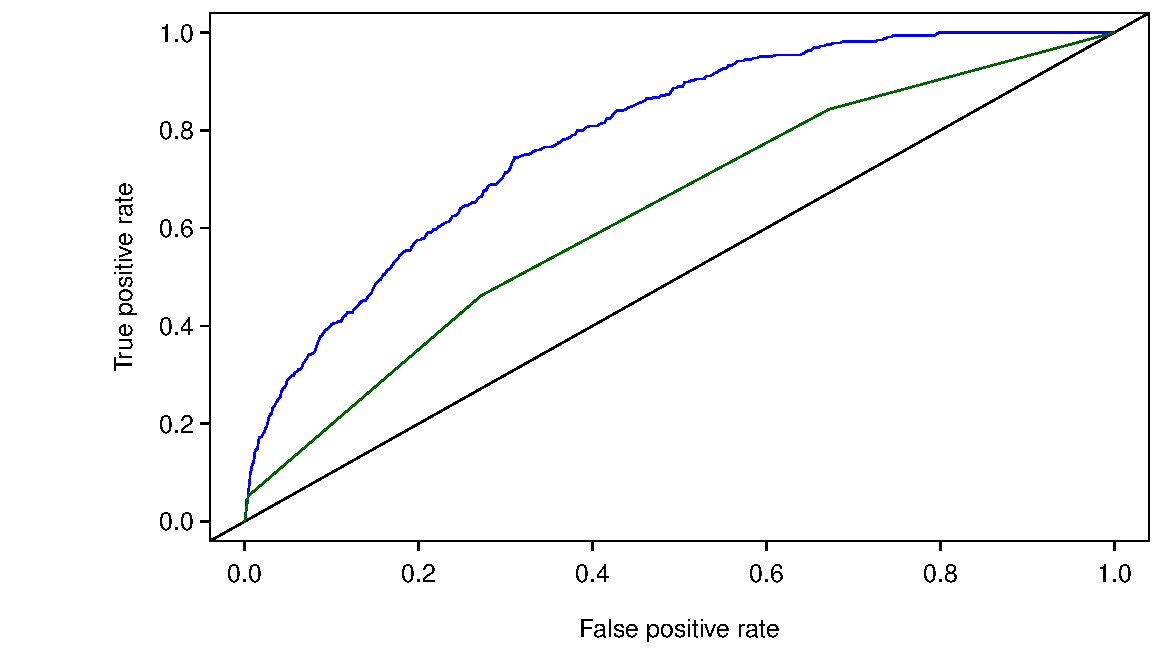
\includegraphics[width=0.70\textwidth]
  {ch_logistic_regression_oi_biostat/figures/ROCDanishED/ROCDanishED.pdf}
    \caption{Receiver operating curves (ROC) for predicting 30-day mortality,  green for the DEPT triage system, blue for the model that adds age and sex to DEPT\@.  The black line is the is 45-degree line $y = x$.}
    \label{figure:ROCDanishED}
\end{figure}

\textD{\newpage}

\subsection{Summary}
\label{section:interpretationNewColorScore}

The ED triage model explored here study illustrates the steps used in building and evaluating a prediction model.   The analysis makes compromises, however, that limit its practical value.  A more complete modification of the DEPT scoring should start by using the predictors used to construct DEPT, add age and sex to those predictors and construct a model based on the full set of predictors.   The analysis here has not used any of the biochemical variables used in the Kristensen paper, many of which are strongly associated with 30-day mortality. The analysis dropped individuals 100 years old or older, rather than exploring transformations of the age variable that might have led to  better fit with the full dataset and to a model that could be applied to all age groups.  Incorporating an age-sex interaction led to a better fitting model, but it is possible that a model without the interaction term would be easier to interpret and still have made reasonably accurate predictions. 

A full analysis would explore some questions raised by the analysis here.  What is the reason for the surprisingly low mortality among the oldest members of the study population? Are they truly more hardy, or are very old patients referred to the ED for different, perhaps less serious conditions and still coded as high-risk?  What might explain the age-sex interaction? 

Despite the caveats, the analysis illustrates aspects that readers should look for in similar analyses. The source of the data should be clearly articulated; steps in model building should be clearly explained; model evaluation should incorporate diagnostic plots whenever  possible and not rely on only numerical  measures of fit.  The predictive ability in models for binary outcome data should always include ROC curves and estimates and confidence intervals for AUC.


\index{data!Danish emergency department (ED|)}
\textD{\newpage}

\section{Notes}
\label{notesLogisticRegression}

This and other chapters use body mass index (BMI) in several examples and analyses because it is widely available and has been measured and recorded in many studies of human populations. Despite its widespread use, BMI is now increasingly questioned because of its potential bias when applied to certain populations.

BMI was first proposed in 1832 by Adolphe Quetelet based on data from Caucasian western Europeans and was originally known as the Quetelet Index. The category labels for BMI were set in 1995 by an expert panel sponsored by WHO but their applicability in Asian and other populations have been questioned and studied.  Several large studies have confirmed that high and low values of BMI in Asians confer an elevated risk of death just as in European populations (for example Lin, et al.\footfullcite{lin2011body}) but did not find evidence that the WHO cutpoints should be adjusted for Chinese populations.   Nevertheless, we chose not to use the current WHO categories when analyzing the hyperuricemia dataset.  In general, labeled categories associated with cutpoints in a continuous predictor should be interpreted with caution.  Chapter 2 of Wiggins and Jones\footnote{Wiggins C and Jones ML.  How Data Happened.  A History from the Age of Reason to the Age of Algorithms (2023).  WW Norton and Company.} describe some of Quetelet's work on BMI and his place in the history of statistics.

The examples using the TB dataset were chosen to illustrate concepts in logistic regression rather than a detailed analysis and examine only the two predictors level of education and presence of MDR TB.  For readers interested in a more in-depth look at the data, the paper by Lackey referenced in Section~\ref{section:logisticChiSqTest} uses logistic regression to examine the association between TB treatment interruption a many more predictors.
